\documentclass[envcountsame,envcountchap, openany, 14pt]{mysvmono2}
% \documentclass[14pt]{report}
\usepackage{blindtext}
\usepackage[paperheight=29.7cm,paperwidth=21.0cm, top=2.5cm, bottom=2cm, left=3.5cm, right=2cm]{geometry}
\usepackage[ddmmyyyy]{datetime}
%!TEX root = book_ML.tex
% \usepackage[margin=1in]{geometry}
\usepackage[T5]{fontenc}
% \setcounter{secnumdepth}{3}
\setcounter{tocdepth}{1} %% depth level of table of content with 0 - chapter only 
\usepackage[utf8]{inputenc}
\usepackage{amsmath}
\usepackage{amssymb}
% \usepackage{amssymb,amsbsy}
% \setlength{\parindent}{0em}
\setlength{\parskip}{1em}
% choose options for [] as required from the list
% in the Reference Guide, Sect. 2.2

% ******************************************************************************
%% force table caption to top 
%https://tex.stackexchange.com/questions/22751/how-to-force-table--on-top
\usepackage{floatrow}
\floatsetup[table]{capposition=top}
\usepackage[font={sf,  }, tableposition=top]{caption}
\usepackage{subcaption}
\DeclareCaptionFormat{rule}{#1#2#3\rule{\textwidth}{.0pt}}
% \DeclareCaptionFormat{norule}{}
\DeclareCaptionLabelFormat{mylabel}{#1 #2.\hspace{1.5ex}}
\captionsetup[figure]{labelformat=mylabel, labelfont = bf, justification=justified, labelsep=none}
%%% change name Table and Figure
\captionsetup[table]{name=Bảng}
\captionsetup[figure]{name=Hình}
% \captionsetup[listing]{name=Code}

% caption on side
\usepackage{floatrow}
\usepackage{sidecap}

% ******************************************************************************


\usepackage{graphicx}        % standard LaTeX graphics tool
% when including figure files
\usepackage{multicol}        % used for the two-column index
\usepackage[bottom]{footmisc}% places footnotes at page bottom
% etc.
% see the list of further useful packages
% in the Reference Guide, Sects. 2.3, 3.1-3.3
% rule after figure
% \usepackage{caption}
% \usepackage[tableposition=top]{caption}

\usepackage{xcolor}
\def\myrule{\textcolor{gray}{\rule{\textwidth}{.1pt}}}
% \def\myrulethin{\rule{\textwidth}{.01pt}}

\usepackage{multirow}
%%%%%%%%%%
\usepackage{makeidx}         % allows index generation
\makeindex             % used for the subject index
% please use the style svind.ist with
% your makeindex program


\usepackage{silence}
\WarningFilter{latex}{Composite letter}
\WarningFilter{latex}{Package hyperref Warning: Composite letter}


\usepackage{cite,url,bm}
% \usepackage{hyperref}
% \urlstyle{rm}
% \usepackage[unicode]{hyperref}
\usepackage[unicode, pdftex,
    pdfauthor={Pham Hong Thai},
    pdftitle={Autoencoders}]{hyperref}
\renewcommand\UrlFont{\sffamily}
\hypersetup{
    colorlinks=black,
    linkcolor=black,
    filecolor=magenta,
    urlcolor=blue,
}

%%%%%%%%%%%%%%%%%%%5
% \usepackage{listings}
% \usepackage{color}
% \usepackage{textcomp}
% %New colors defined below
% \definecolor{codegreen}{rgb}{0,0.6,0}
% \definecolor{codegray}{rgb}{0.5,0.5,0.5}
% \definecolor{codepurple}{rgb}{0.58,0,0.82}
% \definecolor{backcolour}{rgb}{0.95,0.95,0.92}


% \makeatletter
% \expandafter\let\csname active@char\string?\endcsname\relax
% \expandafter\let\csname active@char\string!\endcsname\relax
% \expandafter\let\csname active@char\string:\endcsname\relax


% \initiate@active@char{?}
% \initiate@active@char{!}
% \initiate@active@char{:}
% \makeatletter



\usepackage{courier}

\usepackage{listings}
\renewcommand{\lstlistingname}{Code}
% \usepackage[T1]{fontenc}
\usepackage{xcolor}
\usepackage{textcomp}
%Code listing style named "mystyle"
% \lstdefinestyle{mystyle}{
%   backgroundcolor=\color{backcolour},   commentstyle=\color{codegreen},
%   keywordstyle=\color{magenta},
%   stringstyle=\color{codepurple},
%   basicstyle=\footnotesize,
%   frame = single,
%   breakatwhitespace=false,
%   breaklines=true,
%   captionpos=b,
%   keepspaces=true,
%   numbers=none,
%   numbersep=5pt,
%   showspaces=false,
%   showstringspaces=false,
%   showtabs=false,
%   tabsize=2,
%   basicstyle=\footnotesize\ttfamily,
%   % columns = flexible, 
%   keepspaces = true,
% }

\definecolor{codegreen}{rgb}{0,0.6,0}
\definecolor{codegray}{rgb}{0.5,0.5,0.5}
\definecolor{codepurple}{rgb}{0.58,0,0.82}

\definecolor{codegreen}{rgb}{1, 1, 1}
\definecolor{codegray}{rgb}{.2, .2, .2}
\definecolor{codepurple}{rgb}{0, 0, 0}
\definecolor{codekey}{rgb}{0, 0, 0}
\definecolor{backcolour}{rgb}{1, 1, 1}


\usepackage{courier}

\lstdefinestyle{mystyle}{
    backgroundcolor=\color{backcolour},
    commentstyle=\color{codegray} \itshape,
    keywordstyle=\color{codekey} \bfseries,
    numberstyle=\tiny\color{codekey},
    stringstyle=\color{codepurple},
    basicstyle=\ttfamily\footnotesize\color{codekey},
    % basewidth  = {.5em,0.5em},
    % basicstyle=\ttfamily,
    breakatwhitespace=false,
    breaklines=true,
    captionpos=b,
    keepspaces=true,
    numbers=none,
    numbersep=5pt,
    showspaces=false,
    showstringspaces=false,
    showtabs=false,
    tabsize=4,
    frame = single,
    framesep = 7pt,
    % columns = flexible, 
    % keepspaces = false
}

%"mystyle" code listing set
\lstset{style=mystyle}





\lstset{style=mystyle}
\lstset{basicstyle=\footnotesize\ttfamily,breaklines=true}


% Default fixed font does not support bold face
\DeclareFixedFont{\ttb}{T1}{txtt}{bx}{n}{11} % for bold
\DeclareFixedFont{\ttm}{T1}{txtt}{m}{n}{10}  % for newtcbtheoremal

% Custom colors
% \usepackage{color}
\definecolor{deepblue}{rgb}{0,0,0}
\definecolor{deepred}{rgb}{0,0,0}
\definecolor{deepgreen}{rgb}{0,0,0}


% % Python style for highlighting
\newcommand\pythonstyle{\lstset{
        language=Python,
        basicstyle=\ttm,
        otherkeywords={self},             % Add keywords here
        keywordstyle=\ttb\color{deepblue},
        emph={MyClass,__init__},          % Custom highlighting
        emphstyle=\ttb\color{deepred},    % Custom highlighting style
        stringstyle=\color{deepgreen},
        frame=tb,                         % Any extra options here
        showstringspaces=false            %
    }}


\usepackage{colortbl}

% \include{myenv}
\usepackage{tcolorbox}
\usepackage{wrapfig}
\newtcolorbox{mybox}[3][]
{
    colframe = #2!25,
    colback  = #2!10,
    coltitle = blue,
    title    = \textbf{#3},
    #1,
}



%% ========= long bar notation ==============================
\makeatletter
\newsavebox\myboxA
\newsavebox\myboxB
\newlength\mylenA
\newcommand*\lbar[2][.75]{%
    \sbox{\myboxA}{$\m@th#2$}%
    \setbox\myboxB\null% Phantom box
    \ht\myboxB=\ht\myboxA%
    \dp\myboxB=\dp\myboxA%
    \wd\myboxB=#1\wd\myboxA% Scale phantom
    \sbox\myboxB{$\m@th\overline{\copy\myboxB}$}%  Overlined phantom
    \setlength\mylenA{\the\wd\myboxA}%   calc width diff
    \addtolength\mylenA{-\the\wd\myboxB}%
    \ifdim\wd\myboxB<\wd\myboxA%
        \rlap{\hskip 0.5\mylenA\usebox\myboxB}{\usebox\myboxA}%
    \else
        \hskip -0.3\mylenA\rlap{\usebox\myboxA}{\hskip 0.3\mylenA\usebox\myboxB}%
    \fi}
\makeatother

%%%%%%%%%%%% wide hat 
\def\what{\widehat}



% ******************************************************************************
% custom environments
\tcbuselibrary{theorems}
\tcbuselibrary{skins,raster}
\newtcbtheorem[number within=chapter]{mytheo}{Định lý}{colback=white,colframe=gray,fonttitle=\bfseries}{th}

\newtcbtheorem[number within=chapter]{mydef}{Định nghĩa}{colback=white,colframe=gray,fonttitle=\bfseries}{def}

\newtcbtheorem[number within=chapter]{myalg}{Thuật toán}{colback=white,colframe=gray,fonttitle=\bfseries, fontupper = \itshape}{alg}

% \newenvironment{myalg}
% {
% \begin{tcolorbox}[colback = blue!5, colframe=gray, title = Thuật toán,fonttitle=\bfseries]
% \it
% }
% {
% \end{tcolorbox}
% }

\newenvironment{mydeff}
{
    \begin{tcolorbox}[colback=white,colframe=gray, title = Chú ý,fonttitle=\bfseries]
        \it
        }
        {
    \end{tcolorbox}
}

\newenvironment{mynote}
{
    \begin{tcolorbox}[colback = white!5, colframe=gray, title =,fonttitle=\bfseries]
        \it
        }
        {
    \end{tcolorbox}
}

\newcommand{\newnote}[2]{
    % 1: title, 2: content 
    \begin{tcolorbox}[colback = white, leftrule = .3mm, rightrule = .3mm, toprule = .3mm, bottomrule = .3mm, colframe=black, title =#1,fonttitle=\bfseries]
        \it
        #2
    \end{tcolorbox}
}

\newcommand{\myeqnbox}[1]{
    % 1: content 
    \begin{tcolorbox}[toptitle = 0mm, leftrule = .3mm, rightrule = .3mm, toprule = .3mm, bottomrule = .3mm, colback = white, colframe=black, sharp corners]
        \abovedisplayskip=-10pt
        \belowdisplayskip=-30pt
        #1
    \end{tcolorbox}
}

\renewcommand{\baselinestretch}{1.50}\normalsize

\newenvironment{myfr}
{\begin{center} \it
        \begin{tcolorbox}[colback = yellow!20, colframe=yellow!45!black]
            % \includegraphics[width = 2cm]{logo.png}
            \begin{wrapfigure}{L}{0.1\textwidth}
                \vspace{-100pt}
                \href{https://google.com}{
                    \includegraphics[width=\textwidth]{pgfs/logofundaml.pdf}}
                \vspace{-30pt}
            \end{wrapfigure}
            }
            {
        \end{tcolorbox}
    \end{center}
}
% END custom environments
% ******************************************************************************

% ******************************************************************************
% definitions 
\def\etal{\textit{et al.}}

\def\ba{\mathbf{a}}
\def\bb{\mathbf{b}}
\def\bd{\mathbf{d}}
\def\be{\mathbf{e}}
\def\bm{\mathbf{m}}
\def\bK{\mathbf{K}}
\def\bk{\mathbf{k}}
\def\bM{\mathbf{M}}
\def\bp{\mathbf{p}}
\def\bq{\mathbf{q}}
\def\bx{\mathbf{x}}
\def\by{\mathbf{y}}
\def\bz{\mathbf{z}}
\def\bu{\mathbf{u}}
\def\bv{\mathbf{v}}
\def\bw{\mathbf{w}}

\def\bbx{\bar{\mathbf{x}}}
\def\bbX{\bar{\mathbf{X}}}
\def\bbw{\bar{\mathbf{w}}}

\def\bE{\mathbf{E}}
\def\bX{\mathbf{X}}
\def\bY{\mathbf{Y}}
\def\bZ{\mathbf{Z}}
\def\bA{\mathbf{A}}
\def\bB{\mathbf{B}}
\def\bC{\mathbf{C}}
\def\bP{\mathbf{P}}
\def\bQ{\mathbf{Q}}
\def\bI{\mathbf{W}}
\def\bS{\mathbf{S}}
\def\bT{\mathbf{T}}
\def\bW{\mathbf{W}}
\def\bI{\mathbf{I}}
\def\bL{\mathbf{L}}
\def\bU{\mathbf{U}}
\def\bzero{\mathbf{0}}
\def\bone{\mathbf{1}}
\def\R{\mathbb{R}}
\def\L{\mathcal{L}}
\def\S{\mathcal{S}}


\def\bmt{\left[\begin{matrix}}
            \def\bmt{\end{matrix}\right]}

\def\diag{\text{diag}}

\def\bmt{\left[\begin{matrix}}
            \def\emt{\end{matrix}\right]}

\def\blambda{\boldsymbol{\lambda}}
\def\bxi{\boldsymbol{\xi}}
\def\bSigma{\mathbf{\Sigma}}
\def\bLambda{\boldsymbol{\Lambda}}
\def\bnu{\boldsymbol{\nu}}
\def\bmu{\boldsymbol{\mu}}

% \def\dpcm{\hfill $\square$} % Điều phải chứng minh. 
\def\dpcm{} % Điều phải chứng minh. 
\def\tcr{\textcolor{red}}
\def\tcb{\textcolor{blue}}
\def\trace{\text{trace}}
\def\rank{\text{rank}}
\def\sgn{\text{sgn}}
\def\assign{\leftarrow}
\def\imply{\Rightarrow}
\def\dom{\textbf{dom}}

\def\lg{\textit{\textbf{Lời giải}}:}
\def\vd{\textbf{Ví dụ}: }
\def\kq{{{Kết quả:}}}
% ******************************************************************************

% ******************************************************************************
% Python environment
\lstnewenvironment{python}[1][]
{
    \pythonstyle
    \lstset{#1}
}
{}
% Python for external files
\newcommand\pythonexternal[2][]{{
            \pythonstyle
            \lstinputlisting[#1]{#2}}}
% Python for inline
\newcommand\pythoninline[1]{{\color{deepred}\pythonstyle\lstinline!#1!}}

\newcommand{\bi}[1]{\textit{\textbf{{#1}}}} % bold and italic 
% ******************************************************************************

% ******************************************************************************
%%%%%%%%% Header and {Footer}
\usepackage{fancyhdr}
\pagestyle{fancy}
\fancyhf{}
% \fancyhead[RE,RO]{\nouppercase\leftmark}
% \fancyhead[RE,RO]{\thepage}
\chead{\thepage}
% \fancyhead[RE,LO]{\thepage}
% \fancyfoot[RE,LO]{}
% \fancyfoot[LE,RO]{Trang \thepage}

% \rfoot{Trang \thepage}
% \rfoot{\nouppercase\leftmark}

\fancypagestyle{plain}{%
    \fancyhf{}
    \renewcommand{\headrulewidth}{0pt}
}



\renewcommand{\headrulewidth}{.2pt}
\renewcommand{\footrulewidth}{.1pt}
% ******************************************************************************

\DeclareMathOperator*{\argmin}{argmin}
\DeclareMathOperator*{\argmax}{argmax}



%%%%%% definition

% ******************************************************************************
%%%%%% chapter
\makeatletter
\def\thickhrulefill{\leavevmode \leaders \hrule height 1.2ex \hfill \kern \z@}
\def\@makechapterhead#1{
    \vspace*{10\p@}%
    {\parindent \z@ \centering \reset@font
        \thickhrulefill\quad
        \scshape\bfseries\textit{\@chapapp{}  \thechapter}
        % \scshape\bfseries{\Large CHƯƠNG  \thechapter}
        \quad \thickhrulefill
        \par\nobreak
        \vspace*{10\p@}%
        \interlinepenalty\@M
        \hrule
        \vspace*{10\p@}%
        \Huge \bfseries #1 \par\nobreak
        \par
        \vspace*{10\p@}%
        \hrule
        \vskip 100\p@
    }}
% ******************************************************************************



% ******************************************************************************
% title 
\title{
    % {\centering \bf Machine Learning cơ bản}\\
    \\

    \\
    % {\small First Edition}
    % Lần cập nhật gần nhất:
    \vspace{-1.2cm}
}




\usepackage[compact]{titlesec}
\titlespacing{\section}{0pt}{*0}{*0}
\titlespacing{\subsection}{0pt}{*0}{*0}
\titlespacing{\subsubsection}{0pt}{*0}{*0}
% ******************************************************************************

%% for book cover 
\usepackage{incgraph,tikz}
\usetikzlibrary{patterns}
\newlength{\hatchspread}
\newlength{\hatchthickness}
\newlength{\hatchshift}
\newcommand{\hatchcolor}{}
% declaring the keys in tikz
\tikzset{hatchspread/.code={\setlength{\hatchspread}{#1}},
    hatchthickness/.code={\setlength{\hatchthickness}{#1}},
    hatchshift/.code={\setlength{\hatchshift}{#1}},% must be >= 0
    hatchcolor/.code={\renewcommand{\hatchcolor}{#1}}}
% setting the default values
\tikzset{hatchspread=6pt,
    hatchthickness=0.15pt,
    hatchshift=0pt,% must be >= 0
    hatchcolor=black}
% declaring the pattern
\pgfdeclarepatternformonly[\hatchspread,\hatchthickness,\hatchshift,\hatchcolor]% variables
{custom north west lines}% name
{\pgfqpoint{\dimexpr-2\hatchthickness}{\dimexpr-2\hatchthickness}}% lower left corner
{\pgfqpoint{\dimexpr\hatchspread+2\hatchthickness}{\dimexpr\hatchspread+2\hatchthickness}}% upper right corner
{\pgfqpoint{\dimexpr\hatchspread}{\dimexpr\hatchspread}}% tile size
{% shape description
    \pgfsetlinewidth{\hatchthickness}
    \pgfpathmoveto{\pgfqpoint{0pt}{\dimexpr\hatchspread+\hatchshift}}
    \pgfpathlineto{\pgfqpoint{\dimexpr\hatchspread+0.15pt+\hatchshift}{-0.15pt}}
    \ifdim \hatchshift > 0pt
        \pgfpathmoveto{\pgfqpoint{0pt}{\hatchshift}}
        \pgfpathlineto{\pgfqpoint{\dimexpr0.15pt+\hatchshift}{-0.15pt}}
    \fi
    \pgfsetstrokecolor{\hatchcolor}
    %    \pgfsetdash{{1pt}{1pt}}{0pt}% dashing cannot work correctly in all situation this way
    \pgfusepath{stroke}
}


\tikzstyle{shaded}=[pattern = custom north west lines]

% ******************************************************************************
% section number too close to headers in table of content
% Source: https://tex.stackexchange.com/questions/219160/toc-spacing-between-number-and-header
%
% \usepackage{titletoc}

% \titlecontents{chapter}[0em]{\vspace{.25\baselineskip}}
% {\eqparbox{ch}{\bfseries\thecontentslabel}\enspace}{}
% {\hspace{.5em}\hfill\contentspage}

% \titlecontents{section}[1.8em]{\vspace{.25\baselineskip}}
% {{\thecontentslabel}\enspace}{}
% {\hspace{.5em}\titlerule*[10pt]{$\cdot$}\contentspage}

% \titlecontents{subsection}[4.5em]{\vspace{.25\baselineskip}}
% {\eqparbox{Ss}{\thecontentslabel}\enspace}{}
% {\hspace{.5em}\titlerule*[10pt]{$\cdot$}\contentspage}

% \newcommand*\l@section{\@dottedtocline{1}{1.5em}{2.3em}}
% \newcommand*\l@subsection{\@dottedtocline{2}{3.8em}{3.2em}}
% \newcommand*\l@subsubsection{\@dottedtocline{3}{7.0em}{4.1em}}
% \newcommand*\l@paragraph{\@dottedtocline{4}{10em}{5em}}
% \newcommand*\l@subparagraph{\@dottedtocline{5}{12em}{6em}}

% ******************************************************************************

%%%%%%%%%%%%%
%% Blank page 
%%%%%%%%%%%
\usepackage{afterpage}

\newcommand\blankpage{%
    \null
    \thispagestyle{empty}%
    \addtocounter{page}{-1}%
    \newpage}


%%%%%%%%%%%%%%%%%%%%%%%%%%%%%%%%%%%%%%%%%%%%%%%%%5
% boxed around eqnarray
% source: https://tex.stackexchange.com/questions/109900/how-can-i-box-multiple-aligned-equations

% \newcommand*\widefbox[1]{\fbox{\hspace{2em}#1\hspace{2em}}}

% \usepackage{amsmath}
% \usepackage{empheq}
% \usepackage[theorems,skins]{tcolorbox}

% \newtcolorbox{mymathbox}[1][]{colback=white, sharp corners, #1}

% \usepackage{amsmath}
% add (.) into section number. E.g: 1.1., 1.2., 
\usepackage{titlesec}
\titlelabel{\thetitle.~}
% continous footnote numbering.
\usepackage{chngcntr}
\counterwithout{footnote}{chapter}

\usepackage{enumitem}
% \usepackage{enumerate}
\def\myenum{label=\alph*)}
\setenumerate[0]{label=\alph*.}      

%%%%%% format subsubsection to bold italic
\usepackage{titlesec}
\titleformat*{\subsubsection}{\bfseries\itshape}


\usepackage{natbib}
% \setlength{\bibsep}{5.0pt}
\usepackage{indentfirst}
\usepackage{makecell}
% \usepackage{pbox}
\begin{document}
\frontmatter%%%%%%%%%%%%%%%%%%%%%%%%%%%%%%%%%%%%%%%%%%%%%%%%%%%%%%
\mainmatter%%%%%%%%%%%%%%%%%%%%%%%%%%%%%%%%%%%%%%%%%%%%%%%%%%%%%%%

% %% cover
% \incgraph[documentpaper, overlay={\node[red] at (page.center) {};}][width=\paperwidth]{Chapters/cover/cover1.png}

\section*{\centering Lời cảm ơn}

Lời đầu tiên, em xin bày tỏ sự cảm ơn chân thành đối với Cô giáo, TS.
Nguyễn Thị Mỹ Bình – giáo viên hướng dẫn trực tiếp em.

Em cũng xin gửi lời cảm ơn tới các thầy cô trong khoa Công nghệ thông tin,
trường Đại học Công Nghiệp Hà Nội đã hướng dẫn, chỉ bảo và tạo điều kiện cho em
học tập cũng như nghiên cứu trong thời gian qua.

Cảm ơn Câu lạc bộ HIT, Đội Olympic Tin học khoa Công nghệ thông tin đã đồng hành
cùng em trong suốt quãng thời gian học tập, làm việc tại trường.

Mặc dù đã cố gắng hoàn thành báo cáo nghiên cứu này nhưng chắc chắn
sẽ không tránh khỏi những sai sót, em kính mong nhận được sự thông cảm và chỉ
bảo của các thầy cô và các bạn.

\tableofcontents

%!TEX root = ../book_ML.tex
% \addtocontents{toc}{\protect\newpage}



\index{giảm chiều dữ liệu -- dimensionality reduction}
\index{dimensionality reduction -- giảm chiều dữ liệu}
\index{lựa chọn đặc trưng -- feature selection}
\index{feature selection -- lựa chọn đặc trưng}
\index{trích chọn đặc trưng -- feature extraction}
\index{feature extraction -- trích chọn đặc trưng}

\chapter*{MỞ ĐẦU}
\markboth{Mở đầu}{}
\addcontentsline{toc}{chapter}{MỞ ĐẦU}
\label{part: dimred}

\section{Lý do chọn đề tài}

Với sự phát triển không ngừng của khoa học và công nghệ, đặc biệt là các định dạng phương tiện mới
công nghệ phần cứng thay đổi, cũng như các yêu cầu và loại nội dung đa dạng tạo ra nhu cầu
về các thuật toán nén có giá trị cao hơn các phương pháp nén hiện tại (codec). Chúng em lựa chọn
đề tài này nhằm tìm kiếm, xây dựng, triển khai các phương pháp nén mới tận dụng sự mạnh mẽ
của phần cứng ngày nay.

% Chúng ta sẽ xem xét các phương pháp giảm chiều dữ liệu phổ biến
% nhất: \textit{phân tích thành phần chính} ({principle component analysis}) cho bài toán giảm chiều dữ liệu
% vẫn giữ tối đa lượng thông tin, và \textit{linear discriminant analysis}
% cho bài toán giữ lại những đặc trưng quan trọng nhất cho việc phân loại. Trước
% hết, chúng ta cùng tìm hiểu một phương pháp phân tích ma trận vô
% cùng quan trọng  --  \textit{phân tích giá trị suy biến} ({singular value decomposition}).

\section{Mục đích của đề tài}

\begin{itemize}
      \item Phân tích các kĩ thuật nén cũ (codec)
      \item Xây dựng, tìm kiếm các kĩ thuật, phương pháp mới sử dụng trong nén dữ liệu
            đa phương tiện hiệu quả
      \item Tận dụng sự mạnh mẽ của phần cứng.
\end{itemize}

\section{Đối tượng và phạm vi nghiên cứu của đề tài}
\subsection{Đối tượng}
\begin{itemize}
      \item Các kĩ thuật nén thường được sử dụng (DCT, Huffman, kmean, ... )
      \item Các phương pháp nén được phát triển và thể hiện tính hiệu quả trong thời gian gần đây
      \item Bộ mã hóa tự động (Autoencoder)
      \item Các phương pháp phương pháp đánh giá hiệu năng nén
\end{itemize}
\newpage
\subsection{Phạm vi nghiên cứu}
\begin{itemize}
      \item Tập trung sử dụng bộ dữ liệu tự tạo của các sinh viên trong trường đại học Công nghiệp Hà Nội
      \item Nghiên cứu tập trung chủ yếu các kĩ thuật nén có mất mát dữ liệu.
      \item Tìm kiếm các phương pháp, kĩ thuật nén liên quan đến học máy, học sâu để
            tận dụng khả năng của phần cứng.
\end{itemize}




%!TEX root = ../book_ML.tex

\def\R{\mathbb{R}}
\newpage
\section{Bảng các ký hiệu}
Các ký hiệu sử dụng trong sách được liệt kê trong Bảng~\ref{tab:notation}.

\begin{table}[h]
    \caption{Các quy ước ký hiệu và tên gọi được sử dụng trong báo cáo}
    \label{tab:notation}
    \centering
    \begin{tabular}{|c|l|}
    \hline 
    Ký hiệu & Ý nghĩa  \\ \hline 
    \hline 
    $x, y, N, k$ & in nghiêng, thường hoặc hoa, là các số vô hướng \\ \hline
    $\bx, \by$ & in đậm, chữ thường, là các vector  \\ \hline
    $\bX, \bY$ & in đậm, chữ hoa, là các ma trận  \\ \hline
    $\R$ & tập hợp các số thực \\ \hline 
    $\mathbb{N}$ & tập hợp các số tự nhiên \\ \hline 
    $\mathbb{C}$ & tập hợp các số phức \\ \hline 
    $\R^{m}$ & tập hợp các vector thực có $m$ phần tử \\ \hline 
    $\R^{m\times n}$ &tập hợp các ma trận thực có $m$ hàng, $n$ cột \\ \hline
    $\mathbb{S}^n$ & tập hợp các ma trận vuông đối xứng bậc $n$ \\ \hline 
    $\mathbb{S}^n_{+}$ & tập hợp các ma trận nửa xác định dương bậc $n$ \\
    \hline 
    $\mathbb{S}^n_{++}$ & tập hợp các ma trận xác định dương bậc $n$ \\ \hline 
    $ \in $ & phần tử thuộc tập hợp \\ \hline 
    $ \exists $ & tồn tại \\ \hline 
    $ \forall $ & mọi \\ \hline 
    $ \triangleq$ & ký hiệu là/bởi. Ví dụ $a\triangleq f(x)$ nghĩa là ``ký hiệu
    $f(x)$ bởi $a$''. \\ \hline 
    $x_i$ & phần tử thứ $i$ (tính từ 1) của vector $\bx$ \\ \hline 
    $\sgn(x)$ & hàm xác định dấu. Bằng 1 nếu $x \geq 0$, bằng -1 nếu $x < 0$. \\ \hline
    $\exp(x)$ & $e^x$ \\ \hline
    $\log(x)$ & logarit \textit{tự nhiên} của số thực dương $x$ \\ \hline
    $\displaystyle \argmin_xf(x)$ & giá trị của $x$ để hàm $f(x)$ đạt giá trị nhỏ nhất \\ \hline 
    $\displaystyle \argmax_xf(x)$ & giá trị của $x$ để hàm $f(x)$ đạt giá trị lớn nhất \\ \hline 
    % $a_{ij}$ & phần tử hàng thứ $i$, cột thứ $j$ của ma trận $\bA$ \\ \hline 
    % $\bA^T$ & chuyển vị của ma trận $\bA$ \\ \hline 
    % $\bA^H$ & chuyển vị liên hợp (Hermitian) của ma trận phức $\bA$ \\ \hline 
    % $\bA^{-1}$ & nghịch đảo của ma trận vuông $\bA$, nếu tồn tại \\ \hline 
    % $\bA^{\dagger}$ & giả nghịch đảo của ma trận không nhất thiết vuông $\bA$ \\
    % \hline 
    % $\bA^{-T}$ & chuyển vị của nghịch đảo của ma trận $\bA$, nếu tồn tại \\ \hline 
    % $\|\bx\|_p$ & $\ell_p$ norm của vector $\bx$ \\ \hline  
    % $\|\bA\|_F$ &  Frobenius norm của ma trận $\bA$ \\ \hline 
    % $ \diag(\bA)$ & đường chéo chính của ma trận $\bA$ \\ \hline 
    % $\trace(\bA)$ & trace của ma trận $\bA$ \\ \hline 
    % $\det(\bA)$ & định thức của ma trận vuông $\bA$ \\ \hline 
    % $\text{rank}(\bA)$ & hạng của ma trận $\bA$ \\ \hline 
    o.w & \textit{otherwise}  --  trong các trường hợp còn lại \\ \hline 
    $\displaystyle\frac{\partial f}{\partial x}$ & đạo hàm của hàm số $f$ theo $x \in \R$ \\ \hline
    $\nabla_{\bx}f$ & gradient của hàm số $f$ theo $\bx$ ($\bx$ là vector hoặc ma trận) \\ \hline 
    $\nabla^2_{\bx}f$ & gradient bậc hai của hàm số $f$ theo $\bx$, còn được gọi là \textit{Hesse} \\ \hline 
    $\odot$ & \makecell{Hadamard product (elemenwise product). Phép nhân từng phần tử \\ của hai vector hoặc ma trận cùng kích thước.} \\ \hline 
    $\propto$ & tỉ lệ với \\ \hline 
    % v.v. & vân vân \\ \hline 
    %%%%%%%
    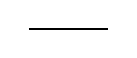
\begin{tikzpicture}
    \draw [thick] (0, 0) -- (1, 0); 
    \end{tikzpicture}
    & đường nét liền \\ \hline 

    %%%%%%%
    \begin{tikzpicture}
    \draw [very thick, dashed] (0, 0) -- (1, 0); 
    \end{tikzpicture}
    & đường nét đứt \\ \hline 

    %%%%%%%
    \begin{tikzpicture}
    \draw [very thick, dotted] (0, 0) -- (1, 0); 
    \end{tikzpicture}
    & đường nét chấm (đường chấm chấm)\\ \hline 

    %%%%%%%
    \begin{tikzpicture}
    \draw [very thick, dash pattern={on 7pt off 2pt on 1pt off 3pt}] (0,0) -- (1,0);
    \end{tikzpicture}
    & đường chấm gạch\\ \hline 
    %%%%%%%
    % \\[-3mm]
    % \vspace{1em}
    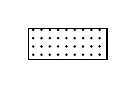
\begin{tikzpicture}[yshift = -1cm]
    \draw [pattern = dots] (0,0) rectangle (1,.4);
    \end{tikzpicture}
    & nền chấm\\\hline 
    %%%%%%%
    % \\[-1em]
    % \vspace{1em}
    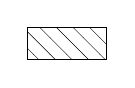
\begin{tikzpicture}
    \draw [pattern = custom north west lines] (0,0) rectangle (1,.4);
    \end{tikzpicture}
    & nền sọc chéo\\ \hline 



    \end{tabular}
 \end{table} 

%!TEX root = ../../book_ML.tex
\chapter{Nghiên cứu tổng quan}
\label{cha: chap1}
% \index{principal component analysis}
% \index{PCA -- \textit{xem} principle component analysis}
% \index{PCA}

% \index{phân tích thành phần chính -- principle component analysis}
% \index{principle component analysis -- phân tích thành phần chính}
% \index{PCA}
\section{Các phương pháp nghiên cứu}

Hiện nay nén dữ liệu được chia thành 2 loại:
\begin{itemize}
      \item Nén không mất mát thông tin
      \item Nén có mất mát thông tin
\end{itemize}

\section{Ưu nhược điểm của các phương pháp}
\subsection{Nén không mất mát thông tin: }

Các thuật toán nén không mất dữ liệu thường dựa trên giả thuyết dư thừa trong dữ liệu
và thể hiện dữ liệu chính xác hơn mà không mất các thông tin. Nén mà không làm mất dữ
liệu là khả thi vì tất cả các dữ liệu thực tế đều có dư thừa. Ví dụ một hình ảnh có thể
có các vùng màu sắc không thay đổi trong nhiều pixel. Thay vì ghi nhận từng pixel
như đỏ, đỏ, đỏ... dữ liệu có thể được ghi là 279 điểm ảnh đỏ liên tiếp. Đây là một
ví dụ về run-length encoding; ngoài ra còn có rất nhiều giải thuật khác.

Dựa theo mức áp dụng thuật toán nén người ta chia nén thành các dạng sau:
\begin{itemize}
      \item Nén tệp tin: Đây là dạng thức nén truyền thống và thuật toán nén được
            áp dụng cho từng tệp tin riêng lẻ. Tuy vậy nếu 2 tệp tin giống nhau thì vẫn
            được nén 2 lần và được ghi 2 lần. Chỉ các byte trùng lắp trong 1 file được loại
            trừ để giảm kích thước. Tùy dữ liệu nhưng thông thường khả năng giảm sau khi
            nén chỉ từ 2-3 lần.
      \item Loại trừ trùng lắp file: Đây là dạng thức nén mà thuật toán nén được
            áp dụng cho nhiều tập tin. Các file giống hệt nhau sẽ chỉ được lưu một lần.
            Ví dụ một thư điện tử có tệp tin đính kèm được gửi cho 1000 người. Chỉ có một
            bản đính kèm được lưu và vì vậy có thể giảm khá nhiều. Thông thường có thể giảm
            từ 5-10 lần so với dữ liệu gốc. - Loại trừ trùng lắp ở mức sub-file: Đây là một
            dạng thức kết hợp cả nén tệp tin và loại trừ trùng lắp
\end{itemize}


\subsection{Nén có mất mát dữ liệu:}

Nén mất dữ liệu giảm số lượng bit bằng cách xác định các thông tin không cần thiết
và loại bỏ chúng.

Chuẩn nén tín hiệu số gồm có các chuẩn sau:

\begin{itemize}
      \item Chuẩn MJPEG:
            Đây là một trong những chuẩn cổ nhất mà hiện nay vẫn sử dụng. MJPEG (Morgan JPEG). Chuẩn này hiện chỉ sử dụng trong các thiết bị DVR rẻ tiền, chất lượng thấp. Không những chất lượng hình ảnh kém, tốn tài nguyên xử lý, cần nhiều dung lượng ổ chứa, và còn hay làm lỗi đường truyền.
      \item Chuẩn MPEG2:
            Chuẩn MPEG là một chuẩn thông dụng. Đã được sử dụng rộng rãi trong hơn một thập kỉ qua. Tuy nhiên, kích thước file lớn so với những chuẩn mới xuất hiện gần đây, và có thể gây khó khăn cho việc truyền dữ liệu.
      \item Chuẩn MPEG-4:
            Mpeg-4 là chuẩn cho các ứng dụng MultiMedia. Mpeg-4 trở thành một tiêu chuẩn cho nén ảnh kỹ thuật truyền hình số, các ứng dụng về đồ hoạ và Video tương tác hai chiều (Games, Videoconferencing) và các ứng dụng Multimedia tương tác hai chiều (World Wide Web hoặc các ứng dụng nhằm phân phát dữ liệu Video như truyền hình cáp, Internet Video...). Mpeg-4 đã trở thành một tiêu chuẩn công nghệ trong quá trình sản xuất, phân phối và truy cập vào các hệ thống Video. Nó đã góp phần giải quyết vấn đề về dung lượng cho các thiết bị lưu trữ, giải quyết vấn đề về băng thông của đường truyền tín hiệu Video hoặc kết hợp cả hai vấn đề trên.
      

\end{itemize}

\subsection{Kết luận}

Vì sự đa dạng cũng như đã được phát triển nhiều của các phương pháp nén có mất mát nên chúng em
đã lựa chọn loại nén này làm chủ đề nghiên cứu chính cho đề tài. 


%!TEX root = ../../book_ML.tex
\chapter{Cơ sở lý thuyết}
\label{cha: chap2}
% \index{principal component analysis}
% \index{PCA -- \textit{xem} principle component analysis}
% \index{PCA}

% \index{phân tích thành phần chính -- principle component analysis}
% \index{principle component analysis -- phân tích thành phần chính}
% \index{PCA}
\section{Tổng quan về các kĩ thuật nén mất mát thông tin}
Trong công nghệ thông tin, nén mất mát thông tin hoặc nén không thể đảo
ngược là lớp phương pháp mã hóa dữ liệu sử dụng các phép gần đúng
và loại bỏ một phần dữ liệu để thể hiện nội dung. Các kỹ thuật này
được sử dụng để giảm kích thước dữ liệu để lưu trữ, xử lý và truyền
tải nội dung. Công nghệ nén mất dữ liệu được thiết kế tốt thường
làm giảm kích thước tệp đáng kể trước khi người dùng cuối nhận
thấy sự xuống cấp.

Nén mất dữ liệu được sử dụng phổ biến nhất để nén dữ liệu
đa phương tiện (âm thanh, video và hình ảnh), đặc biệt trong
các ứng dụng như phương tiện truyền trực tiếp hoặc điện thoại internet.

Để mô tả định lượng mức độ gần đúng của dữ liệu tái tạo so
với dữ liệu gốc, cần có một số hình thức đo độ biến dạng.
Vậy nên, trước khi tìm hiểu về các thuật toán nén mất dữ
liệu thường sử dụng, chúng ta cần quan tâm đến một số hình
thức đo độ biến dạng.

Một phép đo sự biến dạng là 1 đại lượng toán học chỉ mức
độ gần đúng so với giá trị ban đầu của nó sử dụng một số
tiêu chí biến dạng. Khi nhìn vào dữ liệu đã nén, người ta
thường nghĩ về sự khác biệt số giữa dữ liệu gốc và dữ liệu
được tái tạo. Tuy nhiên, khi dữ liệu được nén là một ảnh,
phép đo như vậy có thể không mang lại một kết quả như mong muốn.

Ví dụ: nếu hình ảnh được tái tạo giống với ảnh gốc ngoại
trừ việc nó bị lệch sang phải bởi một đường quét dọc, thì
một người quan sát bình thường sẽ gặp khó khăn trong việc
phân biệt nó với ảnh gốc và do đó sẽ kết luận rằng sự biến
dạng nhỏ. Tuy nhiên, khi tính toán được thực hiện bằng số,
chúng ta nhận thấy sự biến dạng lớn, do những thay đổi lớn
trong các pixel riêng lẻ của ảnh được tái tạo. Vấn đề là
chúng ta cần một phép đo về sự biến đổi cảm giác, chứ không
phải một phương pháp số học ngờ nghệch.

Trong số rất nhiều phép đo biến dạng cảm giác đã được tìm ra,
chúng ta trình bày ba phép đo phổ biến nhất được sử dụng
trong nén hình ảnh. Nếu chúng ta quan tâm đến sự khác nhau
pixel trung bình, thì sai số bình phương(MSE- Mean square error)
$\sigma^2$ thường được sử dụng :

\begin{equation}
    \sigma^2 =  \frac{1}{N} \sum_{n=1}^{N} {\left( {X_n-Y_n} \right)}^2
\end{equation}

Với $X_n$, $Y_n$, $N$ lần lượt là chuỗi dữ liệu vào, chuỗi dữ liệu phục hồi,
độ dài của chuỗi dữ liệu

\section{Các kĩ thuật nén codec thường được sử dụng}

Mã hóa biến đổi(Transform coding), một số hình thức nén mất dữ liệu có thể được coi là ứng dụng
của mã hóa biến đổi , là một kiểu nén dữ liệu được sử dụng cho
hình ảnh kỹ thuật số tín hiệu , âm thanh kỹ thuật số và video kỹ thuật số .

Việc chuyển đổi thường được sử dụng để cho phép lượng tử
hóa tốt hơn (nhắm mục tiêu hơn). Kiến thức về ứng dụng được
sử dụng để chọn thông tin cần loại bỏ, do đó làm giảm băng
thông của nó. Thông tin còn lại sau đó có thể được nén thông
qua nhiều phương pháp. Khi đầu ra được giải mã, kết quả có
thể không giống với đầu vào ban đầu, nhưng được mong đợi là
đủ gần với mục đích của ứng dụng.

\subsection{Phương pháp biến đổi Cosin rời rạc}

Biến đổi Cosin rời rạc (Discrete Cosine Transform - DCT)
là một kỹ thuật mã hóa biến đổi được sử dụng rộng rãi,
có khả năng thực hiện mối tương quan của tín hiệu đầu vào
theo cách độc lập với dữ liệu.

\subsection{Biến đổi Karhunen-Loeve}

\section{Mạng nơ-ron nhân tạo}

\section{Bộ mã hóa tự động (Autoencoder)}

Bộ mã hóa tự động là một kỹ thuật học tập không có giám sát,
trong đó chúng em tận dụng mạng nơ-ron cho nhiệm vụ của học để biểu diễn các tập
giá trị dưới dạng nén, học cách để giải mã dữ liệu từ dạng nén.

Cụ thể, chúng em sẽ thiết kế một kiến trúc mạng nơ-ron nhân tạo sau đó áp đặt một
nút thắt cổ chai trong mạng - điều này đại diện cho sự nén lại một cách tự động.
Mạng này sẽ phải biểu diễn tri thức đầu vào dưới dạng các biểu diễn trong ít
chiều không gian hơn, đây chính là biểu diễn nén của đầu vào.

\begin{figure}
    \begin{subfigure}{0.8\textwidth}
        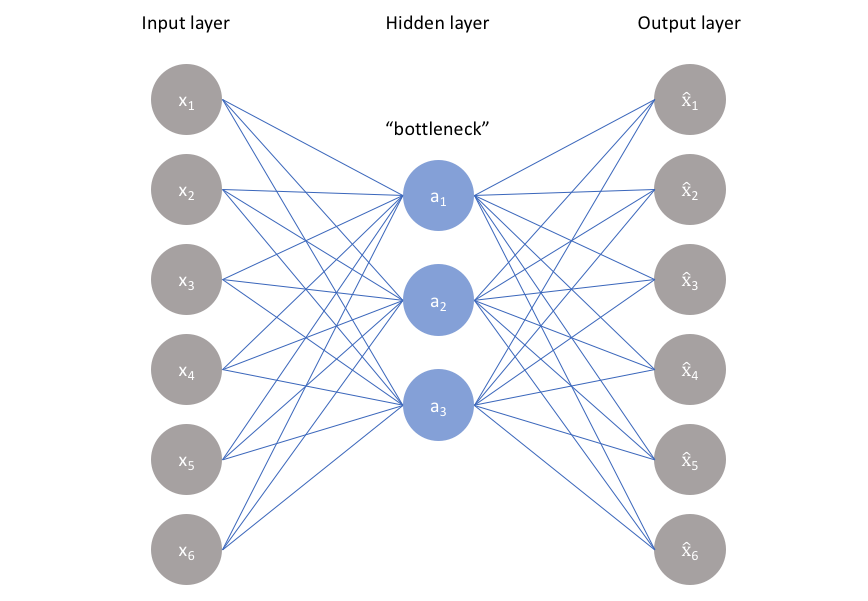
\includegraphics[width=1.0\linewidth]{Chapters/items/autoencoder1.png}
        \caption{}
        \label{fig: auto1}
    \end{subfigure}
    \caption{Bộ mã hóa tự động.}
\end{figure}

\newpage
Nếu các tính năng đầu vào từng độc lập của nhau, việc nén này và tái tạo sau đó sẽ là
một nhiệm vụ rất khó khăn. Tuy nhiên, nếu một số loại cấu trúc tồn tại trong dữ liệu
(ví dụ như: mối tương quan giữa các tính năng đầu vào), cấu trúc này có thể được
học và do đó được tận dụng khi buộc đầu vào thông qua nút thắt cổ chai của mạng.

Bộ mã hóa tự động lý tưởng cân bằng những điều sau đây:
\begin{itemize}[leftmargin=1.5cm]
    \item Nhạy cảm với các yếu tố đầu vào đủ để xây dựng lại một cách chính xác.
    \item Đủ nhạy cảm với các đầu vào mà mô hình không chỉ đơn giản là ghi
          nhớ hoặc trang bị quá nhiều dữ liệu đào tạo.
\end{itemize}

\newpage
Sự đánh đổi này buộc mô hình chỉ duy trì các biến thể trong dữ liệu cần
thiết để cấu trúc lại đầu vào mà không giữ lại các phần dư thừa trong đầu vào.
Đối với hầu hết các trường hợp, điều này liên quan đến việc xây dựng một hàm mất mát
trong đó phải thỏa mãn mô hình của chúng ta nhạy cảm với các yếu tố đầu vào
(ví dụ: xây dựng lại 1 hàm mất mát ${\cal L}\left( {x,\hat x} \right)$ và
thêm một chính quy hóa)


\begin{equation}
    {\cal L}\left( {x,\hat x} \right) + regularizer
\end{equation}

Thông thường, sẽ có thêm một tham số tỷ lệ trước thuật ngữ chính quy để chúng ta
có thể điều chỉnh sự cân bằng giữa hai mục tiêu.

Dưới đây chúng em sẽ trình bày về một số kiến trúc của bộ mã hóa tư động
tiêu chuẩn để áp đặt 2 ràng buộc này và điều chỉnh sự cân bằng.


% \newpage
% \subsection{Cấu trúc bộ mã hóa tự động}
% Một bộ mã hóa tự động có 3 thành phần chính : bộ mã hóa f,
% bộ giải mã g, mô hình xác suất Q

\subsection{Bộ mã hóa tự động chưa hoàn chỉnh}

Kiến trúc đơn giản nhất để xây dựng bộ mã hóa tự động là hạn chế số lượng
nút hiện diện trong (các) lớp ẩn của mạng, hạn chế lượng thông tin có
thể truyền qua mạng. Bằng cách sử dụng các hình phạt mạng theo lỗi xây dựng lại,
mô hình của chúng tôi có thể tìm hiểu các thuộc tính quan trọng nhất của dữ
liệu đầu vào và cách tái tạo tốt nhất dữ liệu đầu vào ban đầu từ trạng thái
"được mã hóa". Lý tưởng nhất là bảng mã này sẽ tìm hiểu và mô tả các thuộc
tính tiềm ẩn của dữ liệu đầu vào.

\begin{figure}
    \begin{subfigure}{0.8\textwidth}
        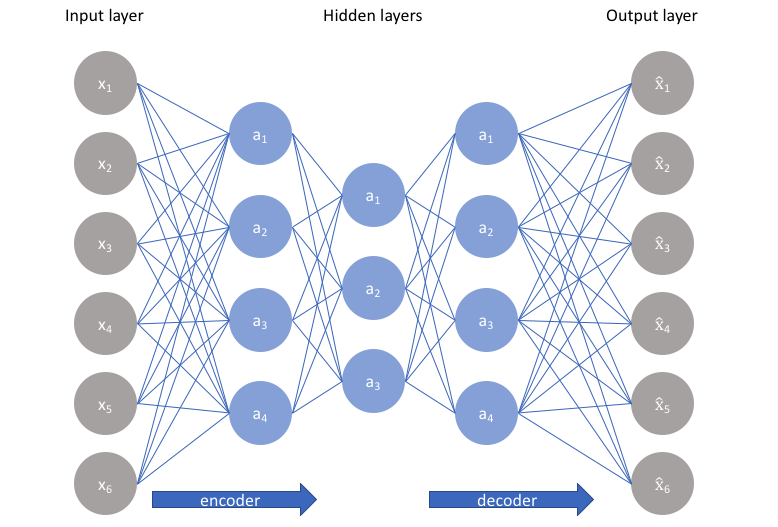
\includegraphics[width=1.\linewidth]{Chapters/items/auto2.jpg}
        \caption{}
        \label{fig: auto2}
    \end{subfigure}
    \caption{Mô tả mô hình bộ mã hóa tự động chưa hoàn chỉnh.}
\end{figure}

Bởi vì mạng nơ-ron có khả năng học các mối quan hệ phi tuyến,
điều này có thể được coi là một sự tổng quát hóa (phi tuyến)
mạnh mẽ hơn của PCA (kĩ thuật giảm chiều dữ liệu tuyến tính)

\newpage
Trong khi PCA cố gắng khám phá một siêu phẳng có chiều thấp hơn
mô tả dữ liệu ban đầu, thì các bộ mã hóa tự động có khả năng học các
đa tạp phi tuyến (đa tạp được định nghĩa theo thuật ngữ đơn giản
là liên tục, không giao nhau bề mặt). Sự khác biệt giữa hai cách
tiếp cận này được hình dung bên dưới.

\begin{figure}
    \begin{subfigure}{0.5\textwidth}
        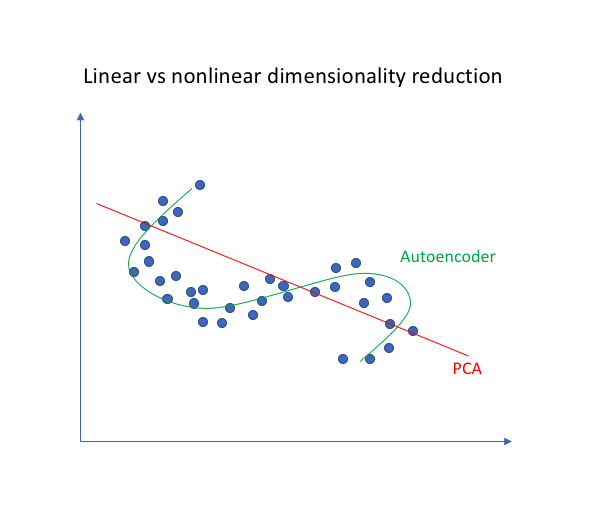
\includegraphics[width=1.\linewidth]{Chapters/items/auto3.jpg}
        \caption{}
        \label{fig: auto3}
    \end{subfigure}
    \caption{Mô tả mô hình bộ mã hóa tự động chưa hoàn chỉnh.}
\end{figure}

Một bộ mã hóa tự động chưa hoàn chỉnh không có thuật ngữ chính quy
rõ ràng - chúng tôi chỉ đào tạo mô hình của mình theo sự mất mát
khi xây dựng lại. Do đó, cách duy nhất của chúng tôi để đảm bảo rằng
mô hình không ghi nhớ dữ liệu đầu vào là đảm bảo rằng chúng tôi đã
hạn chế đủ số lượng các nút trong (các) lớp ẩn.

Đối với các bộ mã hóa tự động sâu, chúng ta cũng phải lưu ý về dung
lượng của bộ mã hóa và các kiểu máy giải mã của chúng ta.
Ngay cả khi "lớp nút cổ chai" chỉ là một nút ẩn, mô hình của
chúng tôi vẫn có thể ghi nhớ dữ liệu huấn luyện với điều kiện là
các mô hình bộ mã hóa và giải mã có đủ khả năng để học một số chức
năng tùy ý có thể ánh xạ dữ liệu thành một chỉ mục.

\subsection{Bộ mã hóa tự động thưa thớt}

Các bộ mã hóa tự động thưa thớt cung cấp cho chúng ta một phương pháp
thay thế để giới thiệu một nút thắt cổ chai thông tin mà không
yêu cầu giảm số lượng nút ở các lớp ẩn của chúng ta. Thay vào đó,
chúng tôi sẽ xây dựng hàm mất mát của chúng tôi để chúng tôi
xử phạt các hàm kích hoạt trong một lớp. Đối với bất kỳ quan sát
nhất định nào, chúng ta sẽ khuyến khích mạng của mình học cách mã hóa và
giải mã chỉ dựa vào việc kích hoạt một số lượng nhỏ nơ-ron.

\begin{figure}
    \begin{subfigure}{0.8\textwidth}
        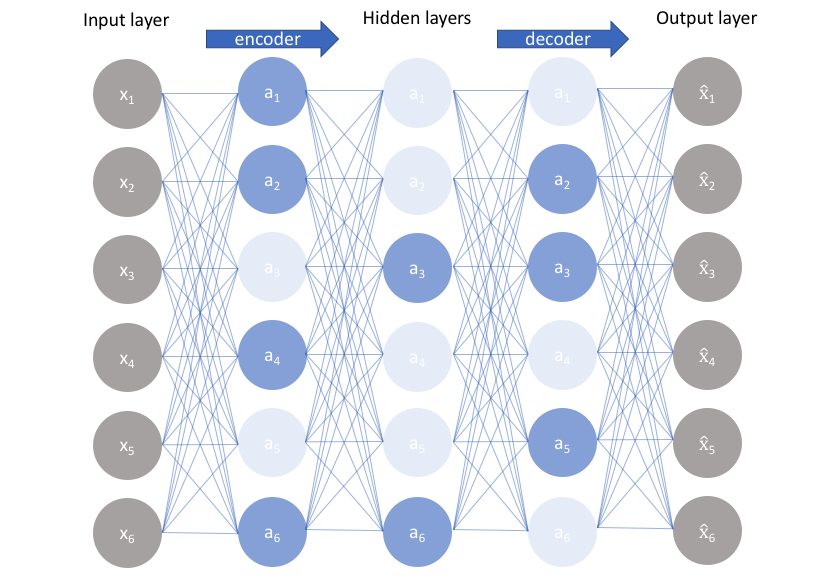
\includegraphics[width=1.\linewidth]{Chapters/items/auto4.jpg}
        \caption{}
        \label{fig: auto4}
    \end{subfigure}
    \caption{Mô tả mô hình bộ mã hóa tự động chưa hoàn chỉnh.}
\end{figure}

\newpage
Một bộ mã hóa tự động thưa thớt chung được hiển thị bên trên nơi
độ mờ của một nút tương ứng với mức độ kích hoạt. Điều quan
trọng cần lưu ý là các nút riêng lẻ của một mô hình được đào
tạo kích hoạt phụ thuộc vào dữ liệu , các đầu vào khác nhau
sẽ dẫn đến việc kích hoạt các nút khác nhau thông qua mạng.

Một kết quả của thực tế này là chúng tôi cho phép mạng của
mình nhạy cảm với các nút lớp ẩn riêng lẻ đối với các thuộc
tính cụ thể của dữ liệu đầu vào. Trong khi một bộ mã hóa tự động
chưa hoàn chỉnh sẽ sử dụng toàn bộ mạng cho mỗi lần quan sát,
một bộ mã hóa tự động thưa thớt sẽ buộc phải kích hoạt có chọn lọc
các vùng của mạng tùy thuộc vào dữ liệu đầu vào. Do đó, chúng
tôi đã giới hạn khả năng ghi nhớ dữ liệu đầu vào của mạng mà
không giới hạn khả năng mạng trích xuất các tính năng từ dữ liệu.

Điều này cho phép chúng tôi xem xét biểu diễn trạng thái tiềm ẩn
và quy định của mạng một cách riêng biệt, do đó chúng tôi có thể
chọn biểu diễn trạng thái tiềm ẩn (tức là kích thước mã hóa) phù
hợp với những gì có ý nghĩa với ngữ cảnh của dữ liệu trong khi áp
đặt chính quy bởi ràng buộc thưa thớt.

Có hai cách chính mà chúng ta có thể áp đặt hạn chế thưa thớt này;
cả hai đều liên quan đến việc đo lường các kích hoạt lớp ẩn
cho mỗi lô đào tạo và thêm một số thuật ngữ vào hàm mất mát để
xử phạt các kích hoạt quá mức. Các cách này là:

\begin{itemize}[leftmargin=1.5cm]
    \item \textbf{L1 Regularization}: Chúng ta có thể thêm một thuật ngữ vào hàm mất mát
          để phạt giá trị tuyệt đối của vector kích hoạt \textit{a} trong lớp \textit{h} với quan sát \textit{i}, được chia tỉ lệ
          bằng 1 tham số điều chỉnh \textit{$\lambda$}
          \begin{equation}
              {\cal L}\left( {x,\hat x} \right) +  \lambda \sum\limits_i {\left| {a_i^{\left( h \right)}} \right|}
          \end{equation}
    \item \textbf{KL-phân kỳ} Về bản chất, KL-phân kỳ là thước đo sự
          khác biệt giữa hai phân phối xác suất. Chúng ta có thể xác định
          tham số thưa thớt \textit{p} biểu thị kích hoạt trung bình của
          một nơ-ron trên một tập hợp các mẫu. Kỳ vọng này có thể được tính là :
          \begin{equation}
              {{\hat \rho }_ j} = \frac{1}{m}\sum\limits_{i} {\left[ {a_i^{\left( h \right)}\left( x \right)} \right]}
          \end{equation}
          trong đó chỉ số con \textit{i} biểu thị nơ-ron cụ thể trong lớp \textit{h}, tính tổng các kích hoạt
          cho các quan sát huấn luyện \textit{m} được ký hiệu riêng lẻ là \textit{x}.

\end{itemize}

\subsection{Bộ mã hóa tự động giảm nhiễu}

Như ở phần giới thiệu, bộ mã hóa tự động chính là một mạng
nơ-ron được đào tạo
trong đó đầu vào giống hệt đầu ra và mô hình có nghiệm vụ tái
tạo đầu vào càng
chặt chẽ càng tốt khi chuyển qua thông tin ở lớp thắt cổ chai.
Một cách tiếp cận khác hướng tới việc phát triển một mô hình
tổng quát hóa là làm nhiễu một chút dữ liệu đầu vào nhưng vẫn
duy trì dữ liệu không bị gián đoạn làm đầu ra mục tiêu của mô hình.

\begin{figure}
    \begin{subfigure}{0.8\textwidth}
        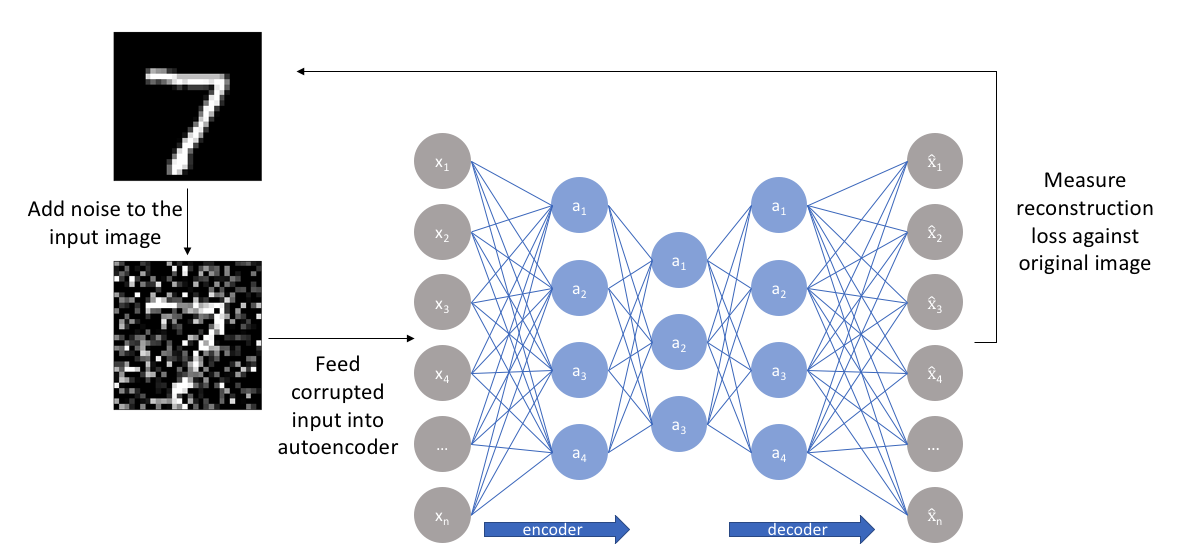
\includegraphics[width=1.\linewidth]{Chapters/items/auto5.jpg}
        \caption{}
        \label{fig: auto5}
    \end{subfigure}
    \caption{Mô tả mô hình bộ mã hóa tự động chưa hoàn chỉnh.}
\end{figure}

Với cách tiếp cận này, mô hình không thể đơn giản
phát triển một ánh xạ ghi nhớ dữ liệu đào tạo vì đầu vào và đầu
ra mục tiêu không còn giống nhau. Thay vào đó, mô
hình học một trường vectơ để ánh xạ dữ liệu đầu vào tới một đa
tạp có chiều thấp hơn (nhớ lại từ hình ảnh trước đây của tôi rằng
một đa tạp mô tả vùng mật độ cao nơi dữ liệu đầu vào tập trung).

\section{Ngôn ngữ lập trình Python và thư viện PyTorch}

\subsection{Ngôn ngữ lập trình Python}

Python là ngôn ngữ lập trình có mục đích chung được bắt đầu bởi Guido van Rossum,
nó trở nên rất phổ biến rất nhanh trong thời gian gần đây, chủ yếu vì tính đơn giản
và khả năng đọc mã của nó. Nó cho phép lập trình viên thể hiện ý tưởng trong ít dòng
mã hơn mà không làm giảm khả năng đọc.

So với các ngôn ngữ như C/C++, Python chậm hơn. Điều đó nói rằng, Python có thể dễ dàng
được mở rộng với C/C++, cho phép chúng ta viết mã chuyên sâu tính toán trong C/C++
và tạo các trình bao bọc Python có thể được sử dụng làm mô-đun Python.
Điều này mang lại cho chúng ta hai lợi thế: thứ nhất, mã nhanh như mã C/C++ gốc
(vì đây là mã C++ thực tế hoạt động ở chế độ nền) và thứ hai, mã dễ dàng hơn trong
Python so với C/C++. OpenCV - Python là một trình bao bọc Python để thực hiện OpenCV C++
ban đầu.

\subsection{Thư viện PyTorch}

PyTorch là một thư viện hỗ trợ tạo ra các mô hình mạng nơ-ron nhân tạo và sử
dụng chúng trong các ứng dụng khác nhau. Trên thực tế PyTorch chính là một
gói hỗ trợ tính toán khoa học (scientific computing) như tài liệu chính
thức của PyTorch đã đề cập

PyTorch, tương tự như Python, nó được thiết kế tập trung vào tính dễ
sử dụng và thậm chí người dùng có kiến thức lập trình rất cơ bản cũng có thể
sử dụng nó trong các dự án có liên quan đến học sâu.



%!TEX root = ../../book_ML.tex
\chapter{Triển khai chương trình và đánh giá hiệu suất}
\label{cha:chap3}
% \index{principal component analysis}
% \index{PCA -- \textit{xem} principle component analysis}
% \index{PCA}

% \index{phân tích thành phần chính -- principle component analysis}
% \index{principle component analysis -- phân tích thành phần chính}
% \index{PCA}
\section{Triển khai chương trình}
Về cơ bản để triển khai một bộ mã hóa tự động cho bài toán nén
có các bước chính sau:
\begin{itemize}[leftmargin=1.5cm]
    \item Thiết kế các lớp mạng
    \item Lựa chọn hàm đánh giá mất mát
    \item Lựa chọn thuật toán tối ưu
    \item Huấn luyện mô hình với tập dữ liệu cần nén
    \item Thực hiện nén, giải nén
\end{itemize}

Hoạt động nén được chia thành 2 quy trình:
\begin{itemize}[leftmargin=1.5cm]
    \item Huấn luyện mô hình (đại diện thao tác nén)
    \item Thực hiện nén, giải nén tập dữ liệu đã huấn luyện
\end{itemize}

\subsection{Thiết kế các lớp mạng}

Kết cấu của mạng này được thiết kế với 50 lớp chia thành 2 phần,
với các lớp tính chập đan xen lớp kích hoạt

\begin{figure}
    \begin{subfigure}{0.8\textwidth}
        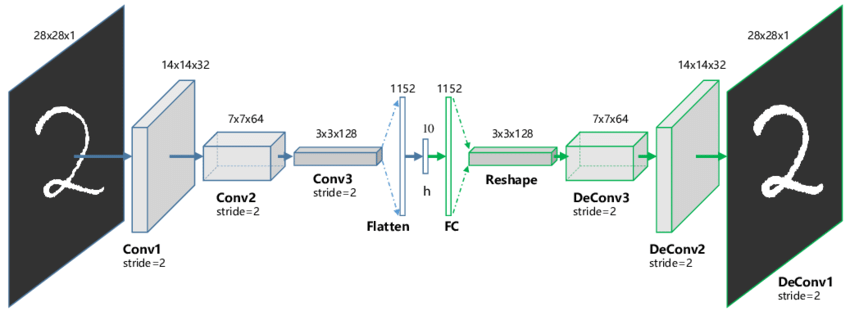
\includegraphics[width=1.\linewidth]{Chapters/items/networks.jpg}
        \caption{}
        \label{fig: net1}
    \end{subfigure}
    \caption{Mô tả mô hình bộ mã hóa tự động đơn giản.}
\end{figure}

Thống kê số lượng tham số trong mạng, tương đương với số lượng các phép tính thực hiện
khi mỗi ảnh được truyền qua mạng.




\subsection{Lựa chọn thuật toán tối ưu}

Các thuật toán tối ưu trong học máy đã phát triển mạnh mẽ từ lâu và đã đạt đến mức hoàn thiện.
Hiện nay có một số thuật toán tối ưu nổi bật như sau :
\begin{itemize}[leftmargin=1.5cm]
    \item Adam là một trong những trình tối ưu hóa phổ biến nhất còn được gọi là Ước tính thời điểm thích ứng, nó kết hợp các thuộc tính tốt của Adadelta và trình tối ưu hóa RMSprop thành một và do đó có xu hướng làm tốt hơn cho hầu hết các vấn đề.
    \item Adagrad (viết tắt của adaptive gradient) xử phạt tốc độ học tập đối với các tham số được cập nhật thường xuyên, thay vào đó, nó cung cấp tốc độ học tập nhiều hơn cho các tham số thưa thớt, các tham số không được cập nhật thường xuyên.
    \item Stochastic gradient descent là cực kỳ cơ bản và hiếm khi được sử dụng bây giờ. Một vấn đề là với tỷ lệ học tập trên toàn thế giới liên quan đến một tương đương. Do đó, nó không hoạt động tốt khi các thông số ở nhiều thang đo vì tốc độ học cà phê sẽ làm cho quá trình đào tạo chậm lại trong khi tốc độ học tập quá lớn có thể gây ra dao động. Ngoài ra, dốc Stochastic đi xuống thường gặp khó khăn khi thoát khỏi các điểm yên ngựa. Adagrad, Adadelta, RMSprop và ADAM thường xử lý các điểm yên ngựa tốt hơn. SGD với xung lượng đưa ra một số tốc độ tối ưu hóa và cũng giúp thoát cực tiểu cục bộ tốt hơn.
\end{itemize}

Nhưng sau khi thực hiện những thử nghiệm nhỏ đơn giản, thì chúng em quyết định
lựa chọn thuật toán tối ưu Adam, là thuật toán đạt độ mất mát thấp và tốc độ hội tụ
để hướng đến nghiệm tối ưu của bài toán tốt.


\subsection{Lựa chọn hàm đánh giá mất mát}

Cũng giông như các thuật toán tối ưu, các hàm đánh giá mất mát cũng đã được phát triển và
hoàn thiện từ lâu, có một số hàm đánh giá nổi bật như sau:
\begin{itemize}
    \item Cross Entropy: Suy hao chéo entropy hay còn gọi là mất log, đo lường hiệu suất của mô hình phân loại có đầu ra là giá
          trị xác suất từ 0 đến 1. Mất entropy chéo tăng lên khi xác suất dự đoán khác với nhãn thực tế. Vì vậy,
          dự đoán xác suất bằng 0,12 khi nhãn quan sát thực tế là 1 sẽ không tốt và dẫn đến giá trị tổn thất cao.
          Một mô hình hoàn hảo sẽ có lỗ nhật ký bằng 0.
    \item Hinge - Thường dùng trong các bài toán phân loại
    \item Huber - Thường được sử dụng để hồi quy. Nó ít nhạy cảm hơn với các ngoại lệ so với MSE vì nó coi lỗi là hình vuông chỉ trong một khoảng thời gian.
    \item MAE, MSE - Là phép tính chuẩn 1, chuẩn 2 thường xuất hiện rất nhiều trong các bài
          toán học máy vì tính đơn giản mà hiệu quả mà nó mang lại.
\end{itemize}

Vì đây là bài toán so sánh độ tương đồng giữa ảnh nên chúng em lựa chọn MSE làm phương pháp đánh giá mất mát cho mô hình


\subsection{Huấn luyện mô hình với tập dữ liệu cần nén}
\subsubsection{Tập dữ liệu sử dụng}

Ở đây, để tăng tính ngẫu nhiên chúng em sử dụng 1 tập dữ liệu ảnh màu với các
kích thước giống nhau (768x1280) được cung cấp từ một thư viện lấy các ảnh ngẫu
nhiên từ các video trên nền tảng Youtube. Với số lượng là 2286 ảnh chất
lượng cao, tổng dung lượng lưa trữ là 6.3 GB

\begin{figure}
    \begin{subfigure}{0.6\textwidth}
        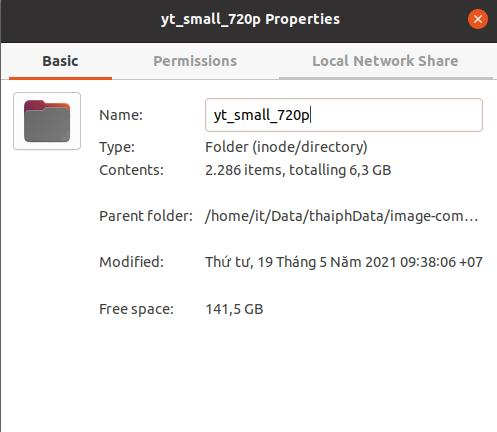
\includegraphics[width=1.\linewidth]{Chapters/items/data.jpg}
        \caption{}
        \label{fig: data}
    \end{subfigure}
    \caption{Tập dữ liệu sử dụng}
\end{figure}

\subsubsection{Các tham số huấn luyện mô hình}
Khi huấn luyện một mô hình mạng nơ-ron nhận tạo điển hình có
các tham số như là : số kỷ nguyên (epoch), Kích thước lô (batch size),
số lân lặp lại (Iterations)

Đối với mô hình này chúng ta phải lựa chọn thêm 1 số tham số giống như
số luồng (thread), tỷ lệ học (learning rate) để mô hình trở lên linh hoạt hơn

Với GPU Tesla T4 16GB, được cung cấp bởi Google Colab và dữ liệu
2286 ảnh chúng em lựa chọn các tham số kích thước lô là 16, số kỷ nguyên là 3,
tỉ lệ học tập là 0,0001, số luồng chạy là 5

\begin{figure}
    \begin{subfigure}{0.7\textwidth}
        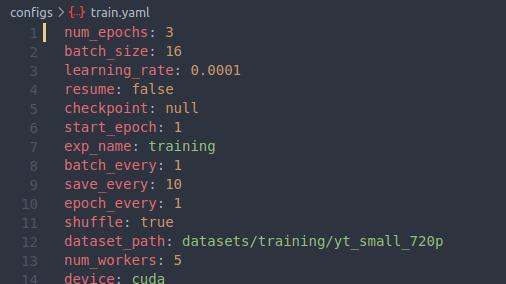
\includegraphics[width=1.\linewidth]{Chapters/items/pram.jpg}
        \caption{}
        \label{fig: param}
    \end{subfigure}
    \caption{Các tham số được lựa chọn}
\end{figure}

\subsubsection{Quá trình huấn luyện mô hình}

Tổng thời gian khi huấn luyện mô hình là khoảng 30 phút, điều này
đại diện cho thời gian nén mặc dù vẫn chưa thực sự tối ưu về mặt
thời gian, nhưng chúng em tin rằng khi phần cứng mạnh mẽ hơn thì
thời gian nén cũng sẽ giảm đi đáng kể.

\begin{figure}
    \begin{subfigure}{0.8\textwidth}
        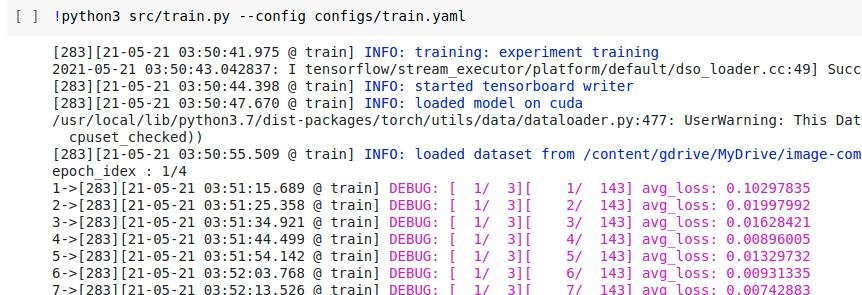
\includegraphics[width=1.\linewidth]{Chapters/items/colab1.jpg}
        \caption{}
        \label{fig: colab1}
    \end{subfigure}
    \caption{Khởi đầu quá trình huấn luyện}
\end{figure}

\newpage
Có thể thấy rằng tham số avg-loss (đánh giá sứ mất mát) từ lúc
bắt đầu huấn luyện cho đến khi kết thúc đã giảm đi rất đáng kể
cho thấy tính đúng đắn của mô hình, dự báo rằng mô hình sẽ đạt kết
quả thử nghiệm tốt.

\begin{figure}
    \begin{subfigure}{0.8\textwidth}
        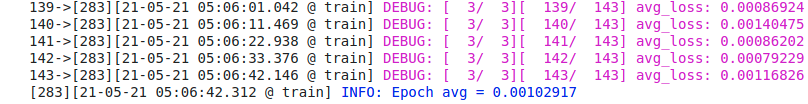
\includegraphics[width=1.\linewidth]{Chapters/items/colab2.jpg}
        \caption{}
        \label{fig: colab2}
    \end{subfigure}
    \caption{Kết thúc quá trình huấn luyện}
\end{figure}

Mô hình hóa quá trình huấn luyện sử dụng tensorboard :
(Trục ngang là số lần lặp lại, trục đứng là đánh giá mất mát)

\begin{figure}
    \begin{subfigure}{0.8\textwidth}
        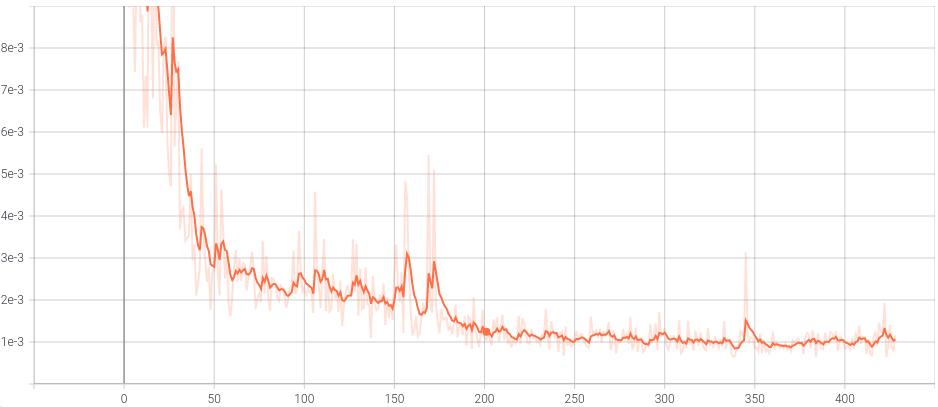
\includegraphics[width=1.\linewidth]{Chapters/items/visualizeTraining.jpg}
        \caption{}
        \label{fig: visualize}
    \end{subfigure}
    \caption{Quá trình giảm của mất mát theo số lần lặp lại các lô}
\end{figure}

\subsection{Thực hiện nén, giải nén}
\section{Đánh giá hiệu suất nén}



%!TEX root = ../../book_ML.tex
\chapter{Kết luận và kiến nghị}
\label{cha:chap4}

\section{Kết luận}
Trên cơ sở tìm hiểu về bài toán nhận diện mặt người trong ảnh, sử dụng pre-trained
model FaceNet được huấn luyện trước trên mạng cơ sở là InceptionResnetV1 do
tiến sĩ khoa học máy tính David Sandberg cung cấp, tôi đã xây dựng thành công hệ
thống điểm danh thông qua hình ảnh khuôn mặt.

Về khả năng phát hiện khuôn mặt, kết quả phát hiện khá tốt hầu hết các trường hợp,
kể cả trong điều kiện thiếu sáng, góc nghiêng, hay có vật che khuất như kính mắt,…

Về khả năng nhận dạng, hệ thống đạt kết quả từ 96-98\% đối với các khuôn mặt thẳng
và điều kiện ánh sáng thích hợp, đạt 92-95\% đối với các khuôn mặt nghiêng hoặc
thiếu sáng.

Về khả năng loại trừ các khuôn mặt “unknown face”, kết quả đạt khoảng 85-90\% khuôn mặt lạ
được phát hiện trong quá trình thử nghiệm.
Hệ thống điểm danh hoạt động ổn định và mượt mà nhờ máy chủ viết bằng Python.
Giao diện được xây dựng trên nền Web là một lợi thế vì tính đơn giản và tiện lợi.

\section{Kiến nghị}

Dựa trên những cơ sở sẵn có này thệ thống có thể được cải tiến trong
tương lai bằng những phương pháp sau:
\begin{itemize}
    \item Cải thiện thời gian chạy của hệ thống, nâng cấp lên có thể chạy trong thời gian thực
    \item Để cải thiện độ chính xác cho hệ thống, đầu tiên ta cần cải thiện bộ dữ liệu dựa trên các tiêu chí như tư thế chụp, góc chụp, hạn chế sự che khuất các bộ phận trên mặt, biểu cảm khuôn mặt, điều kiện ánh sáng, tuổi tác…
    \item Thử nghiệm với nhiều mô hình được huấn luyện trước và thuật toán huấn luyện khác nhau cho bộ dữ liệu của hệ thống.
    \item Thay thế phương pháp loại bỏ khuôn mặt lạ, thử nghiệm và chọn ra ngưỡng cho phép phù hợp hơn.
\end{itemize}

Không chỉ dừng lại ở việc điểm danh, của hệ thống nhận dạng khuôn mặt có thể được sử dụng trong các 
hệ thống mở khóa, thanh toán, hay truy tìm tội phạm,…




% %!TEX root = ../../book_ML.tex
\chapter{Phân tích thành phần chính}
\label{cha:pca}
% \index{principal component analysis}
% \index{PCA -- \textit{xem} principle component analysis}
\index{PCA}

\index{phân tích thành phần chính -- principle component analysis}
\index{principle component analysis -- phân tích thành phần chính}
\index{PCA}
\section{Phân tích thành phần chính}
\subsection{Ý tưởng} % (fold)


% subsection ý_tưởng (end)
%%%%%%% Three subfigures with bottom caption%%%%%%%%%%%%%%
\begin{figure}[t]
    \begin{subfigure}{0.59\textwidth}
        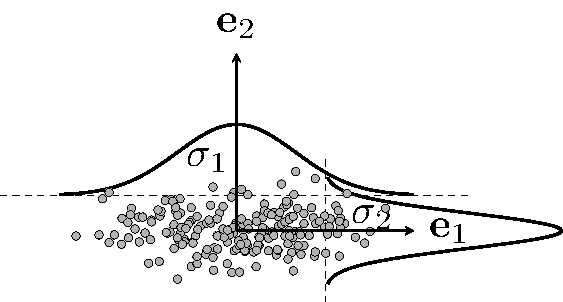
\includegraphics[width=0.99\linewidth]{Chapters/content/27_pca/latex/pca_diagvar.pdf}
         
        \label{fig:pca_2a}
    \end{subfigure}
    \begin{subfigure}{0.33\textwidth}
        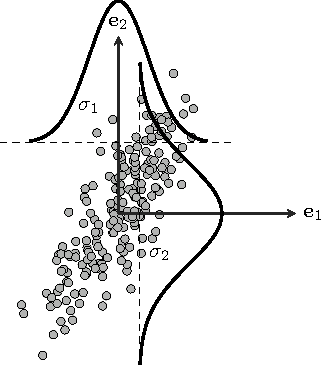
\includegraphics[width=0.99\linewidth]{Chapters/content/27_pca/latex/pca_var0.pdf}
         
        \label{fig:pca_2b}
    \end{subfigure}
    \caption{Ví dụ về phương sai của dữ liệu trong không gian hai chiều. (a)
        Phương sai của chiều thử hai (tỉ lệ với độ rộng của đường hình chuông) nhỏ
        hơn phương sai của chiều thứ nhất. (b) Cả hai chiều có phương sai đáng kể. Phương sai của
        mỗi chiều là phương sai của thành phần tương ứng được lấy trên toàn bộ dữ
        liệu. Phương sai tỉ lệ thuận với độ phân tán của dữ liệu.}
    \label{fig:pca_2}
\end{figure}

Giả sử vector dữ liệu ban đầu $\bx \in \R^{D}$ được giảm chiều trở thành $\bz
    \in \R^K$ với $K < D$. Một cách đơn giản để giảm chiều dữ liệu từ $D$ về $K < D$ là chỉ giữ lại $K$ phần tử {quan trọng nhất}. Có hai câu hỏi lập tức
được đặt ra. Thứ nhất, làm thế nào để xác định {tầm quan trọng} của
mỗi phần tử? Thứ hai, nếu tầm quan trọng của các phần tử là như
nhau, ta cần bỏ đi những phần tử nào?

Để trả lời câu hỏi thứ nhất, hãy quan sát Hình~\ref{fig:pca_2a}. Giả sử các
điểm dữ liệu có thành phần thứ hai (phương đứng) giống hệt nhau hoặc sai khác
nhau không đáng kể (phương sai nhỏ). Khi đó, thành phần này hoàn toàn có thể được lược
bỏ, và ta ngầm hiểu rằng nó sẽ được xấp xỉ bằng kỳ vọng của thành phần đó
trên toàn bộ dữ liệu. Ngược lại, nếu áp dụng phương pháp này lên chiều thứ nhất (phương ngang), {lượng thông tin} bị mất đi đáng kể do sai số xấp xỉ quá lớn. Vì vậy, lượng thông tin theo mỗi thành phần có thể được đo bằng phương sai của dữ liệu trên thành phần đó. Tổng lượng
thông tin là tổng phương sai trên toàn bộ các thành phần. Lấy
một ví dụ về việc có hai camera được đặt dùng để chụp cùng một người, một camera
phía trước và một camera đặt trên đầu. Rõ ràng, hình ảnh thu được từ
camera đặt phía trước mang nhiều thông tin hơn so với hình ảnh nhìn từ
phía trên đầu. Vì vậy, bức ảnh chụp từ phía trên đầu có thể được bỏ qua mà không
làm mất đi quá nhiều thông tin về hình dáng của người đó.

Câu hỏi thứ hai tương ứng với trường hợp Hình~\ref{fig:pca_2b}. Trong cả hai
chiều, phương sai của dữ liệu đều lớn; việc bỏ đi một trong hai chiều đều khiến
một lượng thông tin đáng kể bị mất đi. Tuy nhiên, nếu xoay trục toạ độ đi một
góc phù hợp, một trong hai chiều dữ liệu có thể được lược bở vì dữ liệu có xu
hướng phân bố xung quanh một đường thẳng.

\textit{Phân tích thành phần chính} (principle component analysis, PCA) là
phương pháp đi tìm một phép xoay trục toạ độ để được một hệ trục toạ độ mới sao
cho trong hệ mới này, thông tin của dữ liệu chủ yếu tập trung ở một vài thành
phần. Phần còn lại chứa ít thông tin hơn có thể được lược bỏ.

Phép xoay trục toạ độ có liên hệ chặt chẽ tới hệ trực chuẩn và ma trận trực giao
.Giả sử hệ cơ sở trực chuẩn mới là $\bU$ (mỗi cột của $\bU$ là một vector đơn vị cho
một chiều) và ta muốn giữ lại $K$ toạ độ trong hệ
cơ sở mới này. Không mất tính tổng quát, giả sử đó là $K$ thành phần đầu tiên.
% ******************************************************************************
\begin{figure}[t]
    \centering
    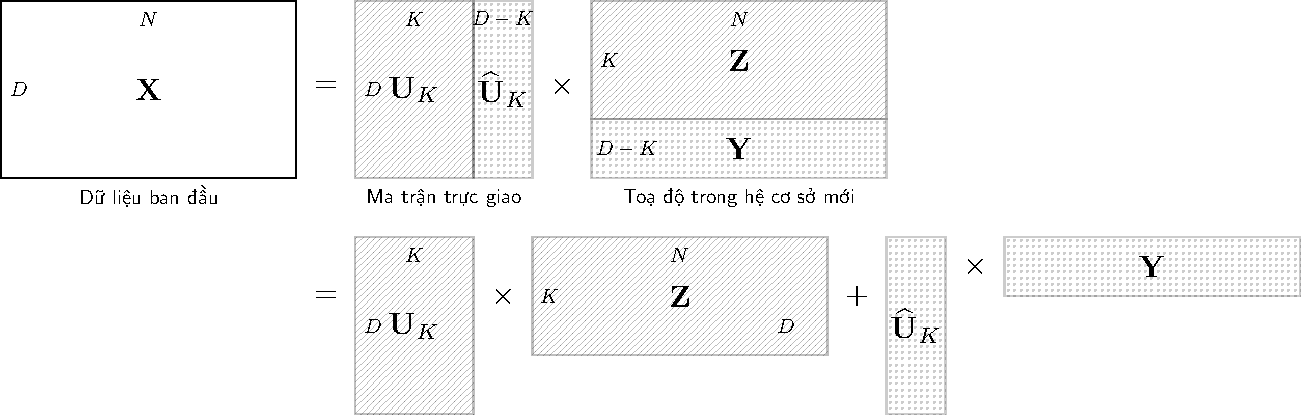
\includegraphics[width = \textwidth]{Chapters/content/27_pca/latex/pca_idea.pdf}
    \caption[]{Ý tưởng chính của PCA: Tìm một hệ trực chuẩn mới sao cho trong hệ này, các thành phần quan trọng nhất nằm trong $K$ thành phần đầu tiên.}
    \label{fig:27_3}
\end{figure}
% ******************************************************************************
Quan sát Hình~\ref{fig:27_3} với cơ sở mới $\bU =
    [\bU_K, \what{\bU}_K]$ là một hệ trực chuẩn với $\bU_K$ là ma trận con tạo bởi $K$ cột đầu tiên của $\bU$. Trong hệ cơ sở mới này, ma trận dữ liệu có thể được viết thành
\begin{equation}
    \label{eqn:27_8}
    \bX = \bU_K \mathbf{Z} + \widehat{\bU}_K \mathbf{Y}
\end{equation}
Từ đây ta cũng suy ra
\begin{eqnarray}
    \label{eqn:27_9}
    \left[\begin{matrix} \mathbf{Z} \\\ \mathbf{Y} \end{matrix} \right] =
    \left[\begin{matrix} \bU_K^T \\\ \what{\bU}_K^T \end{matrix} \right]\bX \Rightarrow
    \begin{matrix}
        \mathbf{Z} = \bU_K^T \bX \\\
        \mathbf{Y} = \what{\bU}_K^T\bX
    \end{matrix}
\end{eqnarray}
Mục đích của PCA là đi tìm ma trận trực giao $\bU$ sao cho phần lớn thông tin
nằm ở $\bU_K \mathbf{Z}$, phần nhỏ thông tin nằm ở $\what{\bU}_K\mathbf{Y}$.
Phần nhỏ này sẽ được lược bỏ và xấp xỉ bằng một ma trận có các
cột như nhau. Gọi mỗi cột đó là
$\mathbf{b}$, khi đó, ta sẽ xấp xỉ $\mathbf{Y} \approx
    \mathbf{b1}^T$ với $\mathbf{1}^T\in \mathbb{R}^{1
        \times N}$ là một vector hàng có toàn
bộ các phần tử bằng một. Giả sử đã tìm được $\bU$, ta cần tìm $\mathbf{b}$ thoả mãn:
\begin{equation}
    \mathbf{b} = \text{argmin}_{\bb} \|\mathbf{Y} - \mathbf{b1}^T\|_F^2 =
    \text{argmin}_{\mathbf{b}} \|\what{\bU}_K^T\bX - \mathbf{b1}^T\|_F^2
\end{equation}
Giải phương trình đạo hàm theo $\mathbf{b}$ của hàm mục tiêu bằng $\bzero$:
\begin{equation}
    (\mathbf{b1}^T - \what{\bU}_K^T\bX)\mathbf{1} = 0 \Rightarrow N\mathbf{b} = \what{\bU}_K^T \mathbf{X1} \Rightarrow \mathbf{b} = \what{\bU}_K^T \lbar{\mathbf{x}}.
\end{equation}
Ở đây ta đã sử dụng $\bone^T\bone = N$ và $\lbar{\bx} = \frac{1}{N}\bX\bone$ là
vector trung bình các cột của $\bX$.
Với giá trị $\mathbf{b}$ tìm được này, dữ liệu ban đầu sẽ được xấp xỉ bởi
\begin{equation}
    \label{eqn:27_10}
    \bX = \bU_K \bZ + \what{\bU}_k\bY \approx \bU_K\bZ + \what{\bU}_k \bb\bone^T
    = \bU_K \mathbf{Z} + \what{\bU}_K \what{\bU}_K^T\bar{\mathbf{x}}\mathbf{1}^T
    \triangleq \tilde{\bX}
    % \bX \approx \tilde{\bX} = \bU_K \mathbf{Z} + \what{\bU}_K \what{\bU}_K^T\bar{\mathbf{x}}\mathbf{1}^T
\end{equation}
\subsection{Hàm mất mát}
Hàm mất mát của PCA được coi như sai số của phép xấp xỉ, được định
nghĩa là
\begin{eqnarray}
    \nonumber
    \frac{1}{N}\|\bX - \tilde{\bX}\|_F^2 &=&
    \frac{1}{N}\|\what{\bU}_K \bY-  \what{\bU}_K
    \what{\bU}_K^T\lbar{\bx}\bone^T\|_F^2 =
    \frac{1}{N}\|\what{\bU}_K \what{\bU}_K^T \bX -  \what{\bU}_K
    \what{\bU}_K^T \bar{\mathbf{x}}\mathbf{1}^T\|_F^2\\
    \label{eqn:27_11}
    &=& \frac{1}{N} \|\what{\bU}_k \what{\bU}_k^T(\bX - \lbar{\bx}\bone^T)\|_F^2
    \triangleq J(\bU)
\end{eqnarray}
Chú ý rằng, nếu các cột của một ma trận $\mathbf{V}$ tạo thành một hệ
trực chuẩn thì với một ma trận $\mathbf{W}$ bất kỳ, ta luôn có
\begin{equation}
    \|\mathbf{VW}\|_F^2 = \text{trace} (\mathbf{W}^T\mathbf{V}^T\mathbf{V} \mathbf{W}) = \text{trace}(\mathbf{W}^T\mathbf{W}) = \|\mathbf{W}\|_F^2
\end{equation}
Đặt $\what{\bX} = \bX - \lbar{\bx}\bone^T$. Ma trận này có được bằng cách trừ
mỗi cột của $\bX$ đi trung bình các cột của nó. Ta gọi $\what{\bX}$ là {ma trận dữ liệu đã
được chuẩn hoá}. Có thể thấy $\hat{\mathbf{x}}_n = \mathbf{x}_n -
    \bar{\mathbf{x}},~\forall n = 1, 2, \dots, N$.

% Ta tạm gọi
% $\what{\bX}$ là ma trận dữ liệu chuẩn hoá.

Vì vậy hàm mất mát trong~\eqref{eqn:27_11} có thể được viết lại thành:
\begin{eqnarray}
    J(\bU) &=&  \frac{1}{N} \|\what{\bU}_K^T\what{\bX} \|_F^2 = \frac{1}{N}
    \|\what{\bX}^T \what{\bU}_K \|_F^2 =
    \frac{1}{N}\sum_{i = K+1}^D \|\what{\bX}^T\mathbf{u}_i \|_2^2 \\\
    \label{eqn:27_12}
    &=& \frac{1}{N} \sum_{i=K+1}^D \mathbf{u}_i^T\what{\bX}\what{\bX}^T \mathbf{u}_i
    = \sum_{i=K+1}^D \mathbf{u}_i^T\mathbf{S} \mathbf{u}_i
\end{eqnarray}
với $\mathbf{S} = \frac{1}{N}\what{\bX}\what{\bX}^T$ là ma trận hiệp phương sai
của dữ liệu và luôn là một ma trận nửa xác định dương.
% (xem Mục~\ref{sub:expectaion_covariance}).

Công việc còn lại là tìm các $\mathbf{u}_i$ để mất mát là nhỏ nhất.

Với ma trận $\bU$ trực giao bất kỳ, thay $K = 0$ vào \eqref{eqn:27_12} ta có
\begin{eqnarray}
    L &=& \sum_{i=1}^D \mathbf{u}_i^T\mathbf{Su}_i = \frac{1}{N} \|\what{\bX}^T\bU\|_F^2 =\frac{1}{N} \text{trace}(\what{\bX}^T\bU \bU^T \what{\bX})  \\\
    \label{eqn:27_13}
    &=& \frac{1}{N} \text{trace} (\what{\bX}^T \what{\bX})  = \frac{1}{N} \text{trace} (\what{\bX} \what{\bX}^T) =\text{trace} (\mathbf{S}) = \sum_{i=1}^D \lambda_i
\end{eqnarray}
Với $\lambda_1 \geq \lambda_2 \geq \dots \geq \lambda_D \geq 0$ là các trị riêng
của ma trận nửa xác định dương $\mathbf{S}$. Chú ý rằng các trị riêng này là
thực và không âm\footnote{Tổng các trị riêng của một ma trận vuông bất kỳ luôn
    bằng vết của ma trận đó.}.


\textit{Như vậy $L$ không phụ thuộc vào cách chọn ma trận trực giao $\bU$} và
bằng tổng các phần tử trên đường chéo của $\mathbf{S}$. Nói cách khác, $L$ chính
là tổng các phương sai theo từng thành phần của dữ liệu ban
đầu\footnote{Mỗi thành phần trên đường chéo chính của ma trận hiệp phương sai
    chính là phương sai của thành phần dữ liệu tương ứng.}.

Vì vậy, việc tối thiểu hàm mất mát $J$ được cho bởi \eqref{eqn:27_12} tương
đương với việc tối đa biểu thức
\begin{equation}
    F  = L - J = \sum_{i=1}^K \mathbf{u}_i \mathbf{S} \mathbf{u}_i^T
\end{equation}
\subsection{Tối ưu hàm mất mát}
Nghiệm của bài toán tối ưu hàm mất mát PCA được tìm dựa trên khẳng định sau
đây:
\newnote{}{
    Nếu $\bS$ là một ma trận nửa xác định dương, bài toán tối ưu
    \begin{eqnarray}
        \max_{\bU_K} \sum_{i=1}^K \bu_i^T\bS\bu_i \\
        \text{thoả mãn:}~ \bU_K^T\bU_K = \bI
    \end{eqnarray}
    có nghiệm $\bu_1, \dots, \bu_K$ là các vector riêng ứng với $K$ trị riêng (kể
    cả lặp) lớn
    nhất của $\bS$. Khi đó, giá trị lớn nhất của hàm mục tiêu là $\sum_{i=1}^K\lambda_i$, với
    $\lambda_1 \geq \lambda_2 \geq \dots \geq \lambda_D$ là các trị riêng của $\bS$.
}

% \textbf{Định lý 1:} $F$ đạt giá trị lớn nhất bằng $\sum_{i=1}^K \lambda_i$ khi $\mathbf{u}_i$ là các vector riêng có norm 2 bằng 1 ứng với các trị riêng này. Tất nhiên, chúng ta không quên điều kiện trực giao giữa các $\mathbf{u}_i$.

% Chú ý rằng $\lambda_i, i = 1, \dots, K$ chính là $K$ trị riêng lớn nhất của ma trận hiệp phương sai $\mathbf{S}$.
Khẳng định này có thể được chứng minh bằng quy nạp
% \footnote
% {Xin được bỏ qua
% phần chứng minh. Bạn đọc có thể xem Excercise 12.1 trong tài liệu tham
% khảo~\cite{bishop2006pattern} với lời giải tại \url{https://goo.gl/sM32pB}.}.

Trị riêng lớn nhất $\lambda_1$ của ma trận hiệp phương sai $\bS$ còn được gọi
là \textit{thành
    phần chính thứ nhất} ({the first principal component}), trị riêng thứ hai
$\lambda_2$ được gọi là \textit{thành phần chính thứ hai},... Tên gọi
\textit{phân tích thành phần chính} ({principal component analysis}) bắt
nguồn từ đây. Ta chỉ giữ lại $K$ thành phần chính đầu tiên khi giảm chiều dữ
liệu dùng PCA.

% ******************************************************************************
\begin{figure}[t]
    % caption on side


    \floatbox[{\capbeside\thisfloatsetup{capbesideposition={right,top},capbesidewidth=7.5cm}}]{figure}[\FBwidth]
    {\caption{ PCA có thể được coi là phương pháp đi tìm một hệ cơ sở trực chuẩn
            đóng vai trò một phép xoay, sao cho trong hệ cơ sở mới này, phương sai theo
            một số chiều nào đó là không đáng kể và có thể lược bỏ. Trong hệ cơ sở ban đầu
            $\mathbf{O}\be_1\be_2$, phương sai theo mỗi chiều (độ rộng của các đường
            hình chuông nét liền) đều lớn. Trong không gian mới với hệ cơ sở
            $\mathbf{O}\bu_1\bu_2$, phương sai theo hai chiều (độ rộng của các đường
            hình chuông nét đứt) chênh lệch nhau đáng kể. Chiều dữ liệu có phương sai nhỏ
            có thể được lược bỏ vì dữ liệu theo chiều này ít phân tán. }
        \label{fig:27_4}}
    { % figure here

        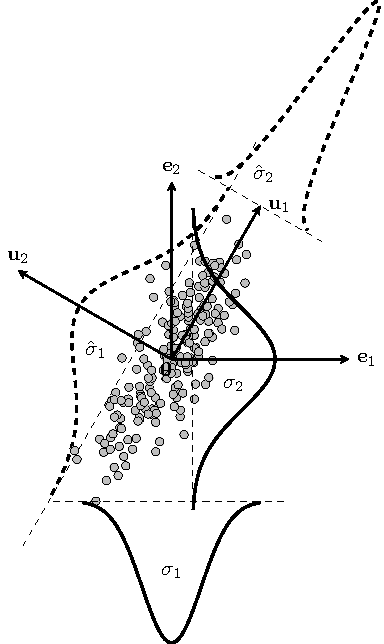
\includegraphics[width=.4\textwidth]{Chapters/content/27_pca/latex/pca_var.pdf}
    }
\end{figure}
% ******************************************************************************
Hình~\ref{fig:27_4} minh hoạ các thành phần chính với dữ liệu hai chiều.
Trong không gian ban đầu với các vector cơ sở $\mathbf{e}_1,
    \mathbf{e}_2$, phương sai theo mỗi chiều dữ liệu (tỉ lệ với độ rộng của các hình chuông
nét liền) đều lớn. Trong hệ cơ sở mới $\mathbf{O}\mathbf{u}_1\mathbf{u}_2$,
phương sai theo chiều thứ hai $\hat{\sigma}_2^2$ nhỏ so với
$\hat{\sigma}_1^2$. Điều này chỉ ra rằng khi chiếu dữ liệu lên $\mathbf{u}_2$, ta
được các điểm rất gần nhau và gần với giá trị trung bình theo chiều đó. Trong
trường hợp này, vì giá trị trung bình theo mọi chiều bằng 0, ta có thể thay thế
toạ độ theo chiều $\mathbf{u}_2$ bằng 0. Rõ ràng là nếu dữ liệu có phương sai
càng nhỏ theo một chiều nào đó thì khi xấp xỉ chiều đó bằng một hằng số, sai số
xấp xỉ càng nhỏ. PCA thực chất là đi tìm một phép xoay tương ứng với một ma trận
trực giao sao cho trong hệ toạ độ mới, tồn tại các chiều có phương sai nhỏ
có thể được bỏ qua; ta chỉ cần giữ lại các chiều/thành phần khác quan trọng hơn. Như
đã khẳng định ở trên, tổng phương sai theo toàn bộ các chiều chiều trong một hệ cơ sở bất kỳ là
như nhau và bằng tổng các trị riêng của ma trận hiệp phương sai. Vì vậy, PCA còn
được coi là phương pháp giảm số chiều dữ liệu sao tổng phương sai còn lại là lớn
nhất.


% Tôi sẽ bỏ qua phần chứng minh của Định lý 1. Tuy nhiên, cũng nêu một vài ý để bạn đọc có thể hình dung:

% Khi $K = 1$. Ta cần giải bài toán:
% \begin{eqnarray}
%     \max_{\mathbf{u}_1} &\mathbf{u}_1^T\mathbf{S} \mathbf{u}_1 \\\
%     \text{thoả mãn:} &\|\mathbf{u}_1\|_2 = 1
% \end{eqnarray}

% Như đã đề cập ở phía trên, hàm mục tiêu đạt giá trị lớn nhất bằng $\lambda_1$ khi $\mathbf{u}_1$ là một vector riêng của ma trận hiệp phương sai $\mathbf{S}$ tương ứng với trị riêng $\lambda_1$. Vậy định lý đúng với $K = 1$

% Giả sử $\mathbf{u}_1$ đã là vector riêng ứng với trị riêng lớn nhất của $\mathbf{S}$ thế thì nghiệm $\mathbf{u}_2$ của bài toán tối ưu:
% \begin{equation}
%     \label{27_21}
%     \begin{aligned}
%     \max_{\mathbf{u}_2} &\mathbf{u}_2^T\mathbf{S} \mathbf{u}_2 \\\
%     \text{thoả mãn:}~ &\|\mathbf{u}_2\|_2 = 1\\\
%     & \mathbf{u}_2^T \mathbf{u}_1 = 0 &
%     \end{aligned}
% \end{equation}
% là một vector riêng của $\mathbf{S}$ ứng với trị riêng lớn thứ hai $\lambda_2$ của nó. Chú ý rằng $\lambda_2$ có thể bằng $\lambda_1$ nếu không gian riêng ứng với $\lambda_1$ có số rank lớn hơn 1.

% Nhận định này có thể được chứng minh bằng phương pháp nhân tử Lagrange. Thật vậy, Lagrangian của bài toán $(21)$ là:
% \begin{equation}
% \mathcal{L}( \mathbf{u}_2, \nu_1, \nu_2) = \mathbf{u}_2^T\mathbf{S} \mathbf{u}_2 + \nu_1\mathbf{u}_1^T\mathbf{u}_2 + \nu_2(1 - \mathbf{u}_2^T\mathbf{u}_2)
% \end{equation}

% Ta cần giải hệ phương trình đạo hàm của $\mathcal{L}$ theo từng biến bằng 0:
% \begin{eqnarray}
%     \label{eqn:27_22}
%     \frac{\partial \mathcal{L}}{\partial \mathbf{u}_2} &=& 2 \mathbf{Su}_2 + \nu_1 \mathbf{u}_1 - 2\nu_2\mathbf{u}_2 = 0\\\
%     \label{eqn:27_23}
%     \frac{\partial \mathcal{L}}{\partial \nu_1} &=& \mathbf{u}_1^T \mathbf{u}_2 = 0 \\\
%     \label{eqn:27_24}
%     \frac{\partial \mathcal{L}}{\partial \nu_2} &=& 1 - \mathbf{u}_2^T \mathbf{u}_2 = 0 \\\
% \end{eqnarray}


% Nhân cả hai vế của \eqref{eqn:27_22} với $\mathbf{u}_1^T$ vào bên trái ta có:
% \begin{equation}
% 2\mathbf{u}_1^T\mathbf{Su}_2 + \nu_1 = 0
% \end{equation}
% Vì $\mathbf{Su}_1 = \lambda_1 \mathbf{u}_1 \Rightarrow \mathbf{u}_1^T\mathbf{Su}_2 = \lambda_1 \mathbf{u}_1^T\mathbf{u}_2 = 0$. Từ đó suy ra $\nu_1 = 0$ và \eqref{eqn:27_22} lúc này tương đương với:
% \begin{equation}
% \mathbf{Su}_2 = \nu_2\mathbf{u}_2 \Rightarrow \mathbf{u}_2^T\mathbf{S} \mathbf{u}_2 = \nu_2
% \end{equation}
% Vậy $\mathbf{u}_2$ là một vector riêng của $\mathbf{S}$ ứng với $\nu_2$. Và để hàm mục tiêu đạt giá trị lớn nhất, $\nu_2$ cần càng lớn càng tốt. Điều này dẫn đến $\nu_2$ phải là trị riêng thứ hai của $\mathbf{S}$.

% Lập luận tương tự, ta có thể chứng minh được: Nếu $\mathbf{u}_i, i = 1, 2, \dots, k-1$ là các vector riêng ứng với trị riêng lớn thứ $i$ của ma trận nửa xác định dương $\mathbf{S}$, hơn nữa, $k-1$ vector riêng này tạo thành một hệ trực chuẩn, thế thì:

% \begin{eqnarray}
%     \max_{\mathbf{u}_k} & \mathbf{u}_k^T\mathbf{Su}_k \\\
%     \text{thoả mãn:}~ & \mathbf{u}_k^T\mathbf{u}_k = 1; \\\
%     & \mathbf{u}_k^T\mathbf{u}_i = 1, i = 1,\dots, k -1
% \end{eqnarray}
% bằng đúng với trị riêng tiếp theo $\lambda_k$ tại $\mathbf{u}_k$ là vector riêng ứng với trị riêng này.



\section{Các bước thực hiện phân tích thành phần chính}
Từ các suy luận trên, ta có thể tóm tắt lại các bước trong PCA như sau:
\begin{itemize}
    \item[1)] Tính vector trung bình của toàn bộ dữ liệu:
          \begin{math}
              \bar{\mathbf{x}} = \frac{1}{N} \sum_{n=1}^N \mathbf{x}_n
          \end{math}.
    \item[2)] Trừ mỗi điểm dữ liệu đi vector trung bình của toàn bộ dữ liệu để được dữ
          liệu chuẩn hoá:
          \begin{equation}
              \hat{\mathbf{x}}_n = \mathbf{x}_n - \bar{\mathbf{x}}
          \end{equation}
    \item[3)] Đặt $\what{\bX} = [\what{\bx}_1, \what{\bx}_2, \dots,
              \what{\bx}_D]$ là ma trận dữ liệu chuẩn hoá, tính ma trận hiệp phương sai:
          \begin{equation}
              \mathbf{S} = \frac{1}{N}\what{\bX}\what{\bX}^T
          \end{equation}
    \item[4)] Tính các trị riêng và vector riêng tương ứng có $\ell_2$ norm bằng 1
          của ma trận này, sắp xếp chúng theo thứ tự giảm dần của trị riêng.
    \item[5)] Chọn $K$ vector riêng ứng với $K$ trị riêng lớn nhất để xây dựng ma trận $\bU_K$ có các cột tạo thành một hệ trực giao. $K$ vector này được gọi là các thành phần chính, tạo thành một không gian con {gần} với phân bố của dữ liệu ban đầu đã chuẩn hoá.
    \item[6)] Chiếu dữ liệu ban đầu đã chuẩn hoá $\what{\bX}$ xuống không gian con tìm được.
    \item[7)] Dữ liệu mới là toạ độ của các điểm dữ liệu trên không gian mới:
          \begin{math}
              \mathbf{Z} = \bU_K^T\what{\bX}
          \end{math}.
\end{itemize}

\textit{Như vậy, PCA là kết hợp của phép tịnh tiến, xoay trục toạ độ và chiếu dữ liệu lên hệ toạ độ mới.}

Dữ liệu ban đầu có thể tính được xấp xỉ theo dữ liệu mới bởi
\begin{math}
    \mathbf{x} \approx \bU_K\mathbf{Z} + \bar{\mathbf{x}}
\end{math}.

Một điểm dữ liệu mới $\bv \in \R^D$ sẽ
được giảm chiều bằng PCA theo công thức $\bw = \bU_K^T(\bv - \lbar{\bx}) \in
    \R^K$. Ngược lại, nếu biết $\bw$, ta có thể xấp xỉ $\bv$ bởi $\bU_K\bw +
    \lbar{\bx}$. Các bước thực hiện PCA được minh hoạ trong Hình \ref{fig:27_5}.

% ******************************************************************************
\begin{figure}[t]
    \centering
    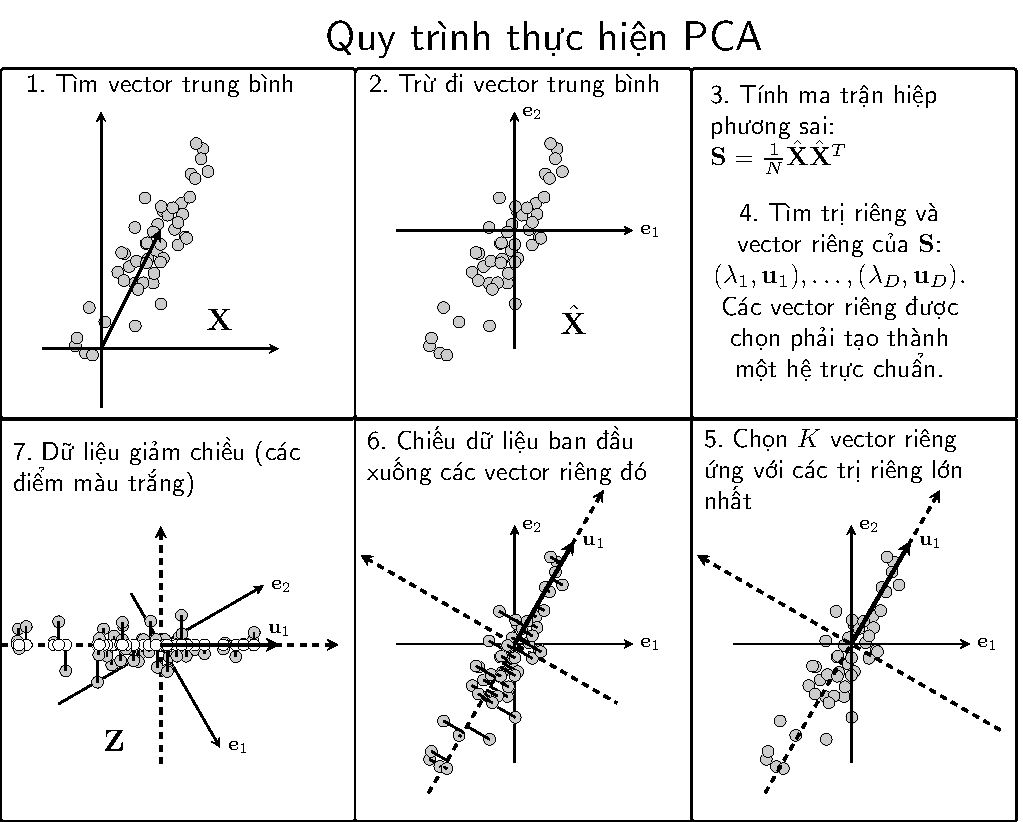
\includegraphics[width = \textwidth]{Chapters/content/27_pca/latex/pca_procedure.pdf}
    \caption[]{Các bước thực hiện PCA.}
    \label{fig:27_5}
\end{figure}
% ******************************************************************************

\section{Liên hệ với phân tích giá trị suy biến}
PCA và SVD có mối quan hệ đặc biệt với nhau. Xin phép nhắc lại hai điểm đã trình bày dưới đây:


\subsection{SVD cho bài toán xấp xỉ hạng thấp tốt nhất}
Nghiệm của bài toán xấp xỉ một ma trận bởi một ma trận có hạng không vượt quá $k$:
\begin{equation}
    \label{eqn:28_1}
    \begin{aligned}
        \min_{\mathbf{A}} & \|\bX - \mathbf{A}\|_F      \\\
        \text{thoả mãn:}~ & \text{rank}(\mathbf{A}) = K
    \end{aligned}
\end{equation}
chính là SVD cắt ngọn của $\mathbf{A}$.

Cụ thể, nếu SVD của $\bX
    \in\mathbb{R}^{D\times N}$ là
\begin{equation}
    \bX = \bU\mathbf{\Sigma}\mathbf{V}^T
\end{equation}
với $\bU \in \mathbb{R}^{D \times D}$ và $\mathbf{V}\in \mathbb{R}^{N\times N}$
là các ma trận trực giao và $\mathbf{\Sigma} \in \mathbb{R}^{D \times N}$ là ma
trận đường chéo (không nhất thiết vuông) với các phần tử trên đường chéo không
âm giảm dần. Nghiệm của bài toán \eqref{eqn:28_1} chính là:
\begin{equation}
    \label{eqn:28_2}
    \mathbf{A} = \bU_K \mathbf{\Sigma}_K \mathbf{V}_K^T
\end{equation}
với $\bU \in \mathbb{R}^{D \times K}$ và $\mathbf{V}\in \mathbb{R}^{N\times K}$
là các ma trận tạo bởi $K$ cột đầu tiên của $\bU$ và $\mathbf{V}$,
$\mathbf{\Sigma}_K \in \mathbb{R}^{K \times K}$ là ma trận đường chéo con ứng
với $K$ hàng đầu tiên và $K$ cột đầu tiên của $\mathbf{\Sigma}$.


\subsection{Ý tưởng của PCA}
Như đã chứng minh ở \eqref{eqn:27_10}, PCA là bài toán đi tìm ma trận
trực giao $\bU$ và ma trận mô tả dữ liệu ở không gian thấp chiều $\mathbf{Z}$
sao cho việc xấp xỉ sau đây là tốt nhất:
\begin{equation}
    \label{eqn:28_3}
    \bX \approx \tilde{\bX} = \bU_K \mathbf{Z} + \what{\bU}_K \what{\bU}_K^T\bar{\mathbf{x}}\mathbf{1}^T
\end{equation}
với $\bU_K, \what{\bU}_K$ lần lượt là các ma trận được tạo bởi $K$ cột đầu tiên
và $D-K$ cột cuối cùng của ma trận trực giao $\bU$, và $\bar{\mathbf{x}}$ là
vector trung bình của dữ liệu.

{Giả sử rằng vector trung bình $\bar{\mathbf{x}} = \mathbf{0}$}. Khi đó, \eqref{eqn:28_3} tương đương với
\begin{equation}
    \label{eqn:28_4}
    \bX \approx \tilde{\bX} = \bU_K \mathbf{Z}
\end{equation}
Bài toán tối ưu của PCA sẽ trở thành:
\begin{equation}
    \label{eqn:28_5}
    \begin{aligned}
        \bU_K, \mathbf{Z} & = & \arg \min_{\bU_K, \mathbf{Z} } \|\bX - \bU_K
        \mathbf{Z}\|_F                                                         \\\
        \text{thoả mãn:}  &   & \bU_K^T \bU_K = \mathbf{I}_K                 &
    \end{aligned}
\end{equation}
với $\mathbf{I}_K \in \mathbb{R}^{K\times K}$ là ma trận đơn vị trong không gian $K$ chiều và điều kiện ràng buộc để đảm bảo các cột của $\bU_K$ tạo thành một hệ trực chuẩn.


\subsection{Quan hệ giữa hai phương pháp}
Có thể nhận ra nghiệm của bài toán \eqref{eqn:28_5} chính là
\begin{align*}
    \bU_K \quad \text{trong}\quad~\eqref{eqn:28_5}     & = \bU_K \quad\text{trong} \quad
    \eqref{eqn:28_2}                                                                                                                 \\\
    \mathbf{Z} \quad\text{trong}\quad~\eqref{eqn:28_5} & = \mathbf{\Sigma}_K \mathbf{V}_K^T \quad\text{trong} \quad \eqref{eqn:28_2}
\end{align*}
Như vậy, nếu các điểm dữ liệu được biểu diễn bởi các cột của một ma trận, và
trung bình các cột của ma trận đó là vector không thì nghiệm của bài toán PCA được rút ra trực tiếp từ SVD cắt ngọn của
ma trận đó. Nói cách khác, việc đi tìm nghiệm cho PCA chính là việc giải một
bài toán phân tích ma trận thông qua SVD.


\section{Làm thế nào để chọn số chiều của dữ liệu mới}

Một câu hỏi được đặt ra là, làm thế nào để chọn giá trị $K$  --  chiều của dữ
liệu mới  --  với từng dữ liệu cụ thể?

Thông thường, $K$ được chọn dựa trên việc {lượng thông tin muốn giữ lại}. Ở đây, toàn bộ thông tin chính là tổng phương sai của toàn bộ các chiều dữ liệu. Lượng dữ liệu muốn dữ lại là tổng phương sai của dữ liệu trong hệ trục toạ độ mới.

Nhắc lại rằng trong mọi hệ trục toạ độ, tổng phương sai của dữ liệu là như nhau
và bằng tổng các trị riêng của ma trận hiệp phương sai $\sum_{i=1}^D
    \lambda_i$. Thêm nữa, PCA giúp giữ lại lượng thông tin (tổng các phương sai) là
$\sum_{i=1}^K \lambda_i$. Vậy ta có thể coi biểu thức:
\begin{equation}
    \label{eqn:28_6}
    r_K = \frac{\sum_{i=1}^K \lambda_i}{\sum_{j=1}^D \lambda_j}
\end{equation}
là tỉ lệ thông tin được giữ lại khi số chiều dữ liệu mới sau PCA là $K$. Như
vậy, giả sử ta muốn giữ lại 99\% dữ liệu, ta chỉ cần chọn $K$ là số tự nhiên
nhỏ nhất sao cho $r_K \geq 0.99$.

Khi dữ liệu phân bố quanh một không gian con, các giá trị phương sai lớn nhất
ứng với các $\lambda_i$ đầu tiên cao gấp nhiều lần các phương sai còn lại.
Khi đó, ta có thể chọn được $K$ khá nhỏ để đạt được $r_K \geq 0.99$.


\section{Lưu ý về tính toán phân tích thành phần chính}
Có hai trường hợp trong thực tế mà chúng ta cần lưu ý về PCA. Trường hợp thứ
nhất là lượng dữ liệu có được nhỏ hơn rất nhiều so với số chiều dữ liệu. Trường
hợp thứ hai là khi lượng dữ liệu trong tập huấn luyện rất lớn, việc tính toán ma trận hiệp phương sai và trị riêng đôi khi trở nên
bất khả thi. Có những hướng giải quyết hiệu quả cho các trường hợp này.

{Trong mục này, ta sẽ coi như dữ liệu đã được chuẩn hoá, tức đã được trừ đi
vector kỳ vọng. Khi đó, ma trận hiệp phương sai sẽ là $\mathbf{S} =
    \frac{1}{N}\bX\bX^T$.}

\subsection{Số chiều dữ liệu nhiều hơn số điểm dữ liệu}

Đó là trường hợp $D > N$, tức ma trận dữ liệu $\bX$ là một \textit{ma trận cao}.
Khi đó, số trị riêng khác không của ma trận hiệp phương sai $\mathbf{S}$ sẽ
không vượt quá hạng của nó, tức không vượt quá $N$. Vậy ta cần chọn $K \leq N$
vì không thể chọn ra được nhiều hơn $N$ trị riêng khác không của một ma trận có hạng
bằng $N$.

Việc tính toán các trị riêng và vector riêng cũng có thể được thực hiện một cách hiệu quả dựa trên các tính chất sau đây:
\begin{enumerate}
    \item  Trị riêng của $\mathbf{A}$ cũng là trị riêng của $k\mathbf{A}$ với $k \neq 0$ bất kỳ. Điều này có thể được suy ra trực tiếp từ định nghĩa của trị riêng và vector riêng.


    \item Trị riêng của $\mathbf{AB}$ cũng là trị riêng của
          $\mathbf{BA}$ với $\mathbf{A} \in \mathbb{R}^{d_1 \times d_2}, \mathbf{B} \in \mathbb{R} ^{d_2 \times d_1}$ là các ma trận bất kỳ và $d_1, d_2$ là các số tự nhiên khác không bất kỳ.

          Như vậy, thay vì tìm trị riêng của ma trận hiệp phương sai $\mathbf{S} \in \mathbb{R}^{D\times D}$, ta đi tìm trị riêng của ma trận $\mathbf{T} = \bX^T \bX \in \mathbb{R}^{N \times N}$ có số chiều nhỏ hơn (vì $N < D$).

    \item Nếu $(\lambda, \mathbf{u})$ là một cặp trị riêng,
          vector riêng của $\mathbf{T}$ thì $(\lambda, \mathbf{Xu})$ là một cặp trị
          riêng, vector riêng của $\mathbf{S}$. Thật vậy:
          \begin{eqnarray}
              \label{eqn:28_8}
              \bX^T \mathbf{Xu} = \bT\bu = \lambda \mathbf{u}
              \Rightarrow (\bX\bX^T)(\mathbf{Xu}) = \lambda (\mathbf{Xu} )
          \end{eqnarray}
          Dấu bằng thứ nhất xảy ra theo định nghĩa của trị riêng và vector riêng.
\end{enumerate}

Như vậy, ta có thể hoàn toàn tính được trị riêng và vector riêng của ma trận
hiệp phương sai $\bS$ dựa trên một ma trận $\bT$ có kích thước nhỏ hơn. Việc
này trong nhiều trường hợp khiến thời gian tính toán giảm đi đáng kể.

% \subsubsection{Chuẩn hoá các vector riêng}

% \textit{Nhắc lại định nghĩa không gian riêng: Không gian riêng ứng với trị riêng của một ma trận là không gian sinh (span subspace) tạo bởi toàn bộ các vector riêng ứng với trị riêng đó.}

% Việc cuối cùng phải làm là chuẩn hoá các vector riêng tìm được sao cho chúng tạo thành một hệ trực chuẩn. Việc này có thể dựa trên hai điểm sau đây:

% \textbf{Thứ nhất}, nếu $\mathbf{A}$ là một ma trận đối xứng, $(\lambda_1,
% \mathbf{x}_1), (\lambda_2, \mathbf{x}_2)$ là các cặp (trị riêng, vector riêng)
% của $\mathbf{A}$ với $\lambda_1 \neq \lambda_2$, thì
% $\mathbf{x}_1^T\mathbf{x}_2 = 0$. Nói cách khác, hai vector bất kỳ trong hai
% không gian riêng khác nhau của một ma trận đối xứng trực giao với nhau.
% Chứng mình:
% \begin{eqnarray}
%   \mathbf{x}_2^T \mathbf{Ax}_1 = \mathbf{x}_1^T \mathbf{Ax}_2 = \lambda_1 \mathbf{x}_2^T \mathbf{x}_1 = \lambda_2 \mathbf{x}_1^T \mathbf{x}_2 \Rightarrow \mathbf{x}_1^T \mathbf{x}_2 = 0
% \end{eqnarray}
% Dấu bằng cuối cùng xảy ra vì $\lambda_1 \neq \lambda_2$.

% \textbf{Thứ hai}, với các trị riêng độc lập tìm được trong một không gian riêng,
% ta có thể dùng quá trình trực giao hoá Gram-Schmit để chuẩn hoá chúng về một hệ
% trực
% chuẩn.

% Kết hợp hai điểm trên, ta có thể thu được các vector riêng tạo thành một hệ trực chuẩn, chính là ma trận $\bU_K$ trong PCA.


\subsection{Với các bài toán quy mô lớn}
Trong rất nhiều bài toán quy mô lớn, ma trận hiệp phương sai là một ma trận rất lớn. Ví dụ, có một triệu bức ảnh
1000 $\times$ 1000 pixel, như vậy $D = N = 10^6$ là các số rất lớn, việc trực
tiếp tính toán trị riêng và vector riêng cho ma trận hiệp phương sai là không
khả thi. Lúc này, các trị riêng và vector riêng của ma trận hiệp phương sai thường được tính thông qua \textit{power method}
(\url{https://goo.gl/eBRPxH}).

\section{Ứng dụng trong nén dữ liệu đa phương tiện dạng ảnh}

\subsection{Triển khai thuật toán PCA bằng ngôn ngữ python}

Để thực hiện triển khai thuật toán chúng ta sẽ thực hiện bằng 6 bước sau :

\begin{itemize}
    \item Tính hiệu giá trị của giá trị mỗi cột và giá trị trung bình của cột đó
    \item Tính ma trận hiệp phương sai dữ liệu
    \item Tính toán giá trị riêng và vector riêng của ma trận hiệp phương sai
    \item Sắp xêp các giá trị riêng theo chiều tăng dần
    \item Chọn tập con trong tập giá trị riêng đã sắp xếp
    \item Chuyển đổi dữ liệu
\end{itemize}

\newpage
Đây là đoạn code thực hiện các bước trên sử dụng ngôn ngữ python và thư viện numpy (1 thư viện hỗ trợ tính toán)
\begin{lstlisting}[language=Python]
    import numpy as np
 
    def PCA(X , num_components):
        
        #Step-1
        X_meaned = X - np.mean(X , axis = 0)
        
        #Step-2
        cov_mat = np.cov(X_meaned , rowvar = False)
        
        #Step-3
        eigen_values , eigen_vectors = np.linalg.eigh(cov_mat)
        
        #Step-4
        sorted_index = np.argsort(eigen_values)[::-1]
        sorted_eigenvalue = eigen_values[sorted_index]
        sorted_eigenvectors = eigen_vectors[:,sorted_index]
        
        #Step-5
        eigenvector_subset = sorted_eigenvectors[:,0:num_components]
        
        #Step-6
        X_reduced = np.dot(eigenvector_subset.transpose() , X_meaned.transpose() ).transpose()
        
        return X_reduced
    
\end{lstlisting}

\
\newpage
\subsection{Chương trình nén sử dụng PCA bằng ngôn ngữ python}
\subsubsection{Mô hình tổng quan của chương trình}

Mô hình tập trung vào chứng minh tính giảm chiều dữ liệu của thuật toán PCA

\begin{center}
    \begin{figure}[htp]
        \begin{center}
            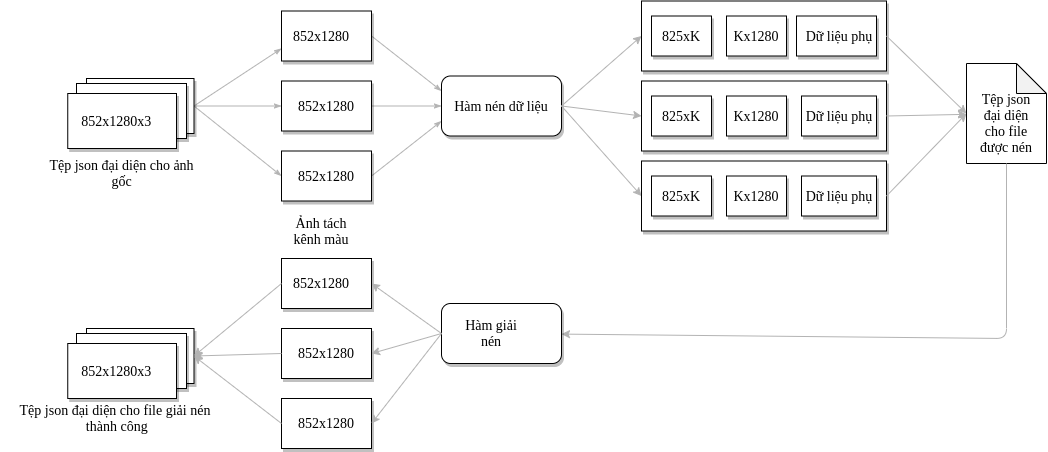
\includegraphics[width=\textwidth,height=\textheight,keepaspectratio]{Chapters/content/27_pca/model.png}
        \end{center}
        \caption{Mô tả chương trình}
        \label{fig:27_6}
    \end{figure}
\end{center}

\subsubsection{Nén và lưu trữ dữ liệu nén}

Hàm sử dụng để nén các ma trận ảnh riêng biệt kích thước mxn:


Hàm này đươc thực thi với các tham số  là ma trận các điểm ảnh và phần trăm nén ảnh.
\newpage
\begin{lstlisting}[language=Python]
    def compress_img(img, percen):
        '''compress image with percent'''

        pca = PCA().fit(img)
        var_cumu = np.cumsum(pca.explained_variance_ratio_)*100
        k = np.argmax(var_cumu > percen)

        ipca = IncrementalPCA(n_components=k)
        img_compressed = ipca.fit_transform(img)
        list_att = ['components_', 'mean_', 'explained_variance_', 'whiten']
        ipca_att = {}
        for att in list_att:
            ipca_att[att] = ipca.__getattribute__(att)
        return k, img_compressed, ipca_att
    
\end{lstlisting}

Kết quả các giá trị mà hàm này trả về :
\begin{itemize}
    \item Số lượng thành phần chính cần thiết để có phần trăm nén tương ứng
    \item Ma trận rút gọn theo các thành phần ở trên
    \item Các tham số cần thiết cho việc phục hồi lại ma trận ban đầu (đương nhiều là ma trận phục hội sẽ bị mất mát dữ liệu)
\end{itemize}

\begin{center}
    \begin{figure}[htp]
        \begin{center}
            
\includegraphics[width=\textwidth,height=\textheight,keepaspectratio]{Chapters/content/27_pca/imgg_origin.jpg}
        \end{center}
        \caption{Ảnh đưa vào bộ nén}
        \label{fig:27_7}
    \end{figure}
\end{center}

\subsubsection{Giải nén từ dữ liệu nén}

Hàm giải nén được thực thi với các tham số truyền vào là các giá trị kết quả của hàm nén

Hàm này chịu trách nghiệm phục hồi lại ảnh với kích thước ban đầu

\begin{lstlisting}[language=Python]
    def extract_img(result_compressed):
        k = result_compressed[0]
        ipca = IncrementalPCA(n_components=k)
        img_compressed = result_compressed[1]
        dict_att = result_compressed[2]
        for key in dict_att.keys():
            ipca.__setattr__(key, dict_att[key])
        # print((dict_att['mean_']))
        img_extracted = ipca.inverse_transform(img_compressed)
        return img_extracted
    
\end{lstlisting}

\subsubsection{Phục hồi ảnh từ các ma trận được giải nén}

Đoạn mã sau thể hiện sự gộp các ma trận của 3 kênh màu RGB từ ảnh ban đầu sau 1 chuỗi xử lý nén và giải nén

\begin{lstlisting}[language=Python]
    # read json file
    img_compressed1 = {}
    with open(path+'imgj_compressed.json', 'r') as f:
        img_compressed1 = json.load(f)

    # extract image
    img_extracted = [extract_img(img_tmp)for img_tmp in img_compressed1]
    img_extracted = concat_img(*img_extracted)
    
\end{lstlisting}

Biến \pythoninline{img_extracted} lưu ảnh hoàn thiện sau khi đã gộp lại từ các ma trận của 3 kênh màu RGB

\begin{center}
    \begin{figure}[htp]
        \begin{center}
            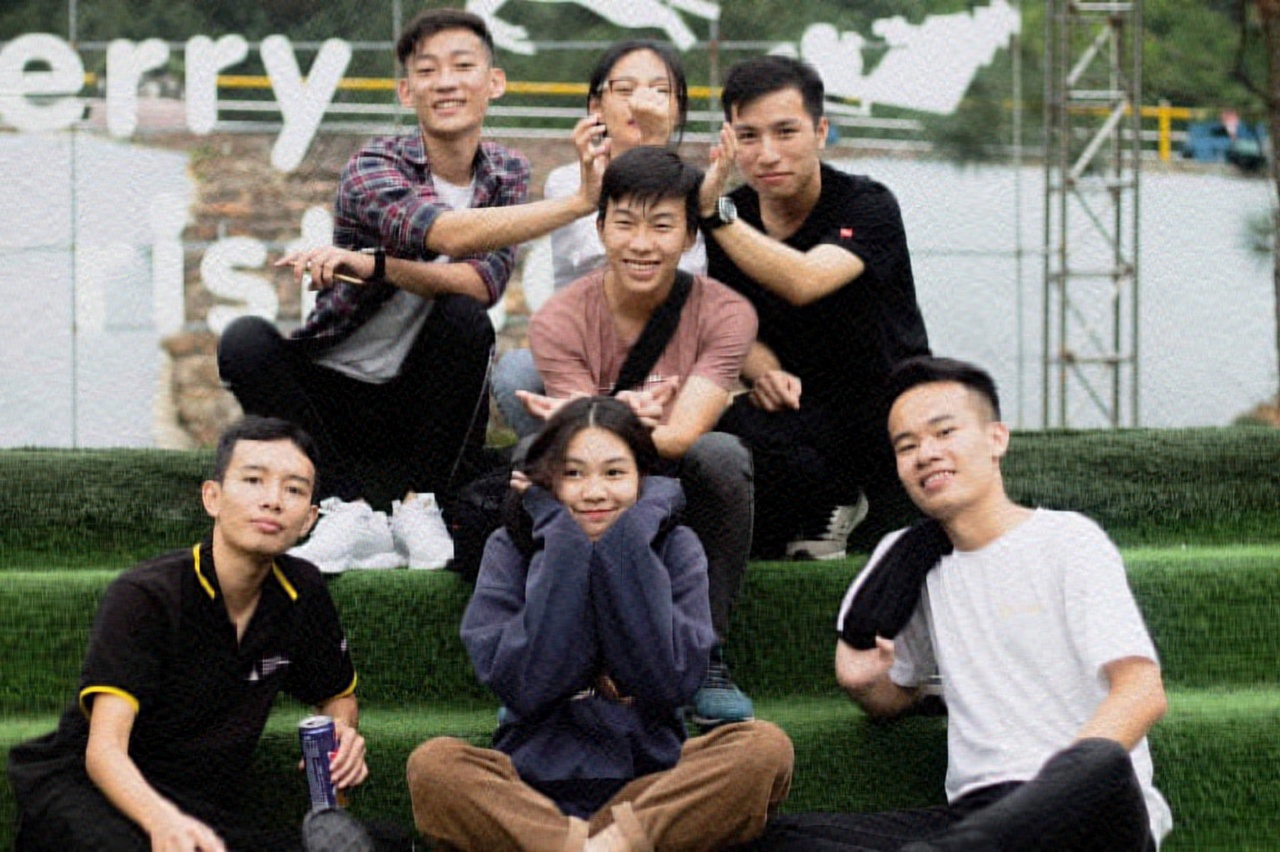
\includegraphics[width=\textwidth,height=\textheight,keepaspectratio]{Chapters/content/27_pca/imgg_extracted.jpg}
        \end{center}
        \caption{Ảnh giải nén sau khi đã được gộp từ các ma trận của 3 kênh màu}
        \label{fig:27_8}
    \end{figure}
\end{center}



\newpage
\subsubsection{Biểu diễn hiệu quả nén}

\begin{center}
    \begin{figure}[htp]
        \begin{center}
            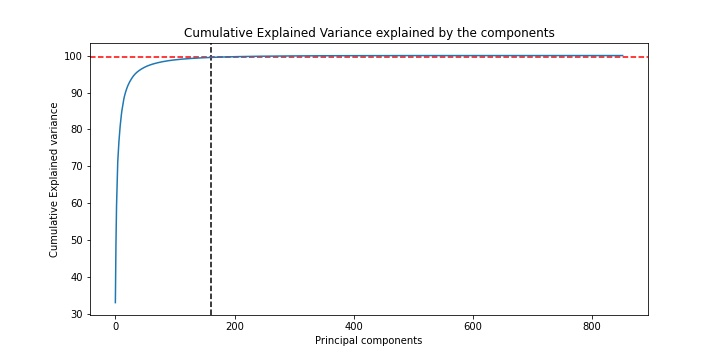
\includegraphics[scale=.5]{Chapters/content/27_pca/cumsum.jpg}
        \end{center}
        \caption{Đường thể hiện tổng cộng dồn của các giá trị riêng thành phần chính}
        \label{fig:27_9}
    \end{figure}
\end{center}

Biểu đồ trên cho thấy khi ta lựa chọn số phần trăm nén là 99$\%$ thì số lượng thành phần được chọn cũng chỉ bằng $1/4$ tổng số thành phần.


Nên khi gặp những ảnh có đường biểu diễn như thế thì hiệu quả nén được sẽ lớn nhưng mất mát thì nhỏ.

\begin{center}
    \begin{figure}[htp]
        \begin{center}
            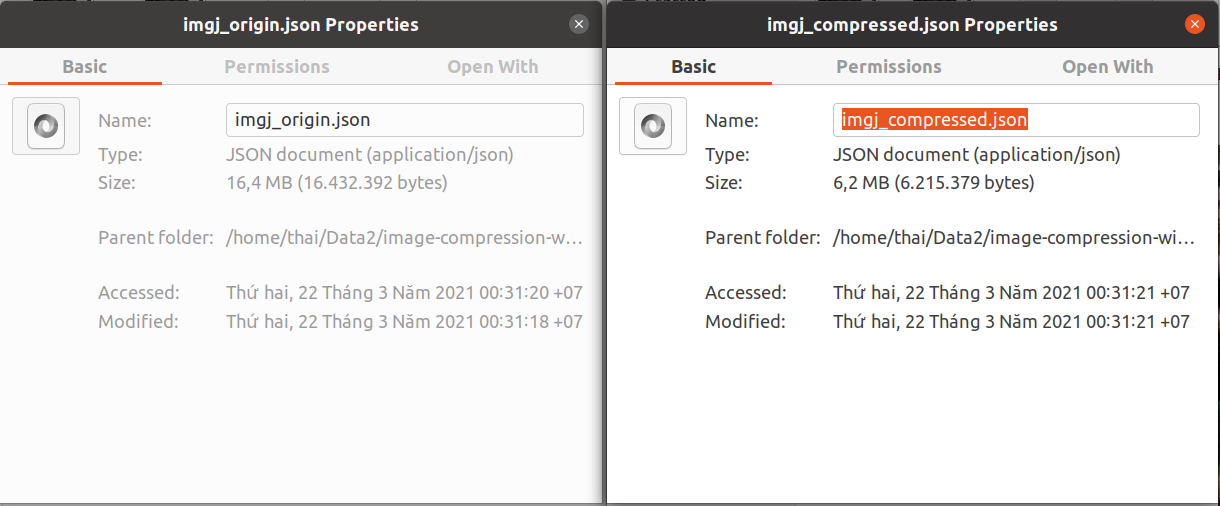
\includegraphics[width=\textwidth,height=\textheight,keepaspectratio]{Chapters/content/27_pca/compare.png}
        \end{center}
        \caption{So sánh tệp trước và sau khi nén}
        \label{fig:27_10}
    \end{figure}
\end{center}

Kết quả chúng ta đã thu được tệp nén có kích thước 6.4 MB so với 16.4 MB của tệp gốc, tức là chỉ bằng $40\%$ so với tệp gốc.
\newpage
\subsubsection{So sánh hiệu quả nén với các định dạng ảnh khác nhau}
\begin{center}
    \begin{figure}[htp]
        \begin{center}
            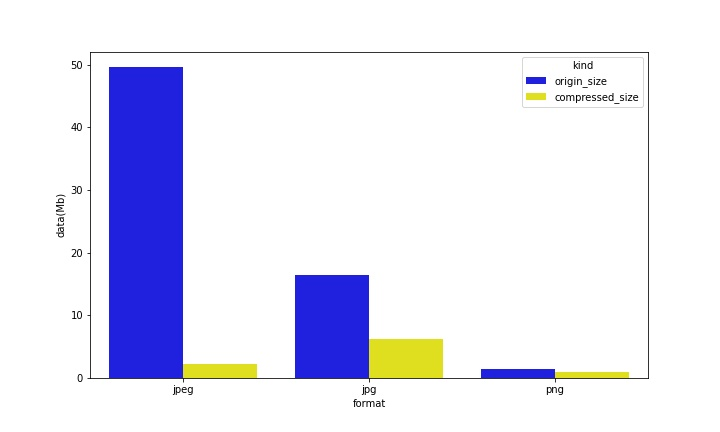
\includegraphics[width=\textwidth,height=\textheight,keepaspectratio]{Chapters/content/27_pca/barplot.jpg}
        \end{center}
        \caption{Đối chiếu kích thước tệp nén và tệp gốc của các định dạng ảnh khác nhau}
        \label{fig:27_11}
    \end{figure}
\end{center}

Chú thích :
\begin{itemize}
    \item Cột màu xanh : dung lượng của file gốc
    \item Cột màu vàng : dung lượng của file nén
\end{itemize}

Kết luận :
\begin{itemize}
    \item Đối với ảnh định dạng jpeg thì hiệu quả nén cao hơn so với các định dạng khác
    \item Đối với ảnh định dạng png thì hiệu quả nén rất thấp do ảnh png là ảnh được tạo thành từ các vector chứ không phải từ những điểm ảnh cố định
\end{itemize}


% \begin{document}
% \centering
% 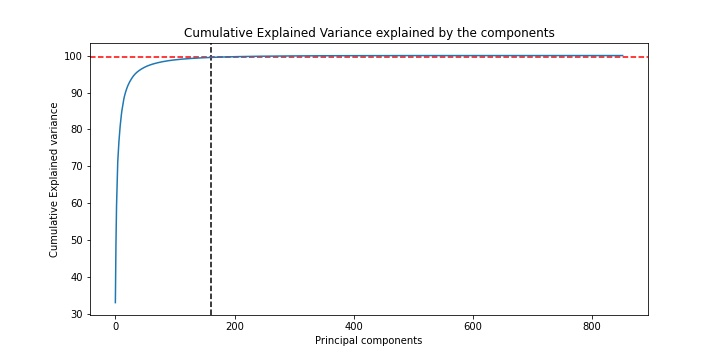
\includegraphics[width = \textwidth]{Chapters/content/27_pca/cumsum.jpg}
% \caption{Ví dụ về ảnh của một người trong Yale Face Database.}
% \end{document}



\section{Một số ứng dụng khác}
Ứng dụng đầu tiên của PCA chính là việc giảm chiều dữ liệu, giúp
việc lưu trữ và tính toán được thuận tiện hơn. Thực tế cho thấy, nhiều khi làm
việc trên dữ liệu đã được giảm chiều mang lại kết quả tốt hơn so với dữ liệu
gốc. Thứ nhất, có thể phần dữ liệu mang thông tin nhỏ bị lược đi chính là phần
gây nhiễu, những thông tin quan trọng hơn đã được giữ lại. Thứ hai, số điểm dữ
liệu nhiều khi ít hơn số chiều dữ liệu. Khi có quá ít dữ liệu và số chiều dữ
liệu quá lớn, quá khớp rất dễ xảy ra. Việc giảm chiều dữ liệu phần nào giúp
khắc phục hiện tượng này.

Dưới đây là hai ví dụ về ứng dụng của PCA trong bài toán phân loại khuôn mặt và dò điểm bất thường.

\subsection{Khuôn mặt riêng}
\index{khuôn mặt riêng -- eigenface}
\index{eigenface -- khuôn mặt riêng}
\textit{Khuôn mặt riêng} (eigenface) từng là một trong những kỹ thuật phổ biến
trong bài toán nhận dạng khuôn mặt. Ý tưởng của khuôn mặt riêng là đi tìm một
không gian có số chiều nhỏ hơn để mô tả mỗi khuôn mặt, từ đó sử dụng vector
trong không gian thấp chiều này như vector đặc trưng cho bộ phân loại. Điều đáng
nói là một bức ảnh khuôn mặt có kích thước khoảng 200 $\times$ 200 sẽ có số
chiều là 40k -- một số rất lớn, trong khi đó, vector đặc trưng thường chỉ có số
chiều bằng vài trăm hoặc vài nghìn. Khuôn mặt riêng thực ra chính là PCA. Các
khuôn mặt riêng chính là các vector riêng ứng với những trị riêng lớn nhất của
ma trận hiệp phương sai.

\index{cơ sở dữ liệu khuôn mặt Yale -- Yale face database}
\index{Yale face database -- cơ sở dữ liệu khuôn mặt Yale}
Trong phần này, chúng ta làm một thí nghiệm nhỏ trên \textit{cơ sở dữ liệu
    khuôn mặt Yale} (\url{https://goo.gl/LNg8LS}). Các bức ảnh trong thí nghiệm
này đã được căn chỉnh cho cùng với kích thước và khuôn mặt nằm trọn vẹn trong
một hình chữ nhật có kích thước $116 \times  98$ điểm ảnh. Có tất cả 15 người khác
nhau, mỗi người có 11 bức ảnh được chụp ở các điều kiện ánh sáng và cảm xúc khác
nhau, bao gồm \pythoninline{'centerlight', 'glasses', 'happy', 'leftlight',
    'noglasses', 'normal', 'rightlight','sad', 'sleepy', 'surprised'}, và
\pythoninline{'wink'}. Hình \ref{fig:28_1} minh hoạ các bức ảnh của
người có id là 10.
% <hr>
% <div class="imgcap">
% <img src ="/assets/28_pca2/yaleb_exs.png" align = "center" width = "800">
% </div>
% <div class = "thecap" align = "left">Hình 1: Ví dụ về ảnh của một người trong Yale Face Database. </div>
% <hr>

\begin{figure}[t]
    \centering
    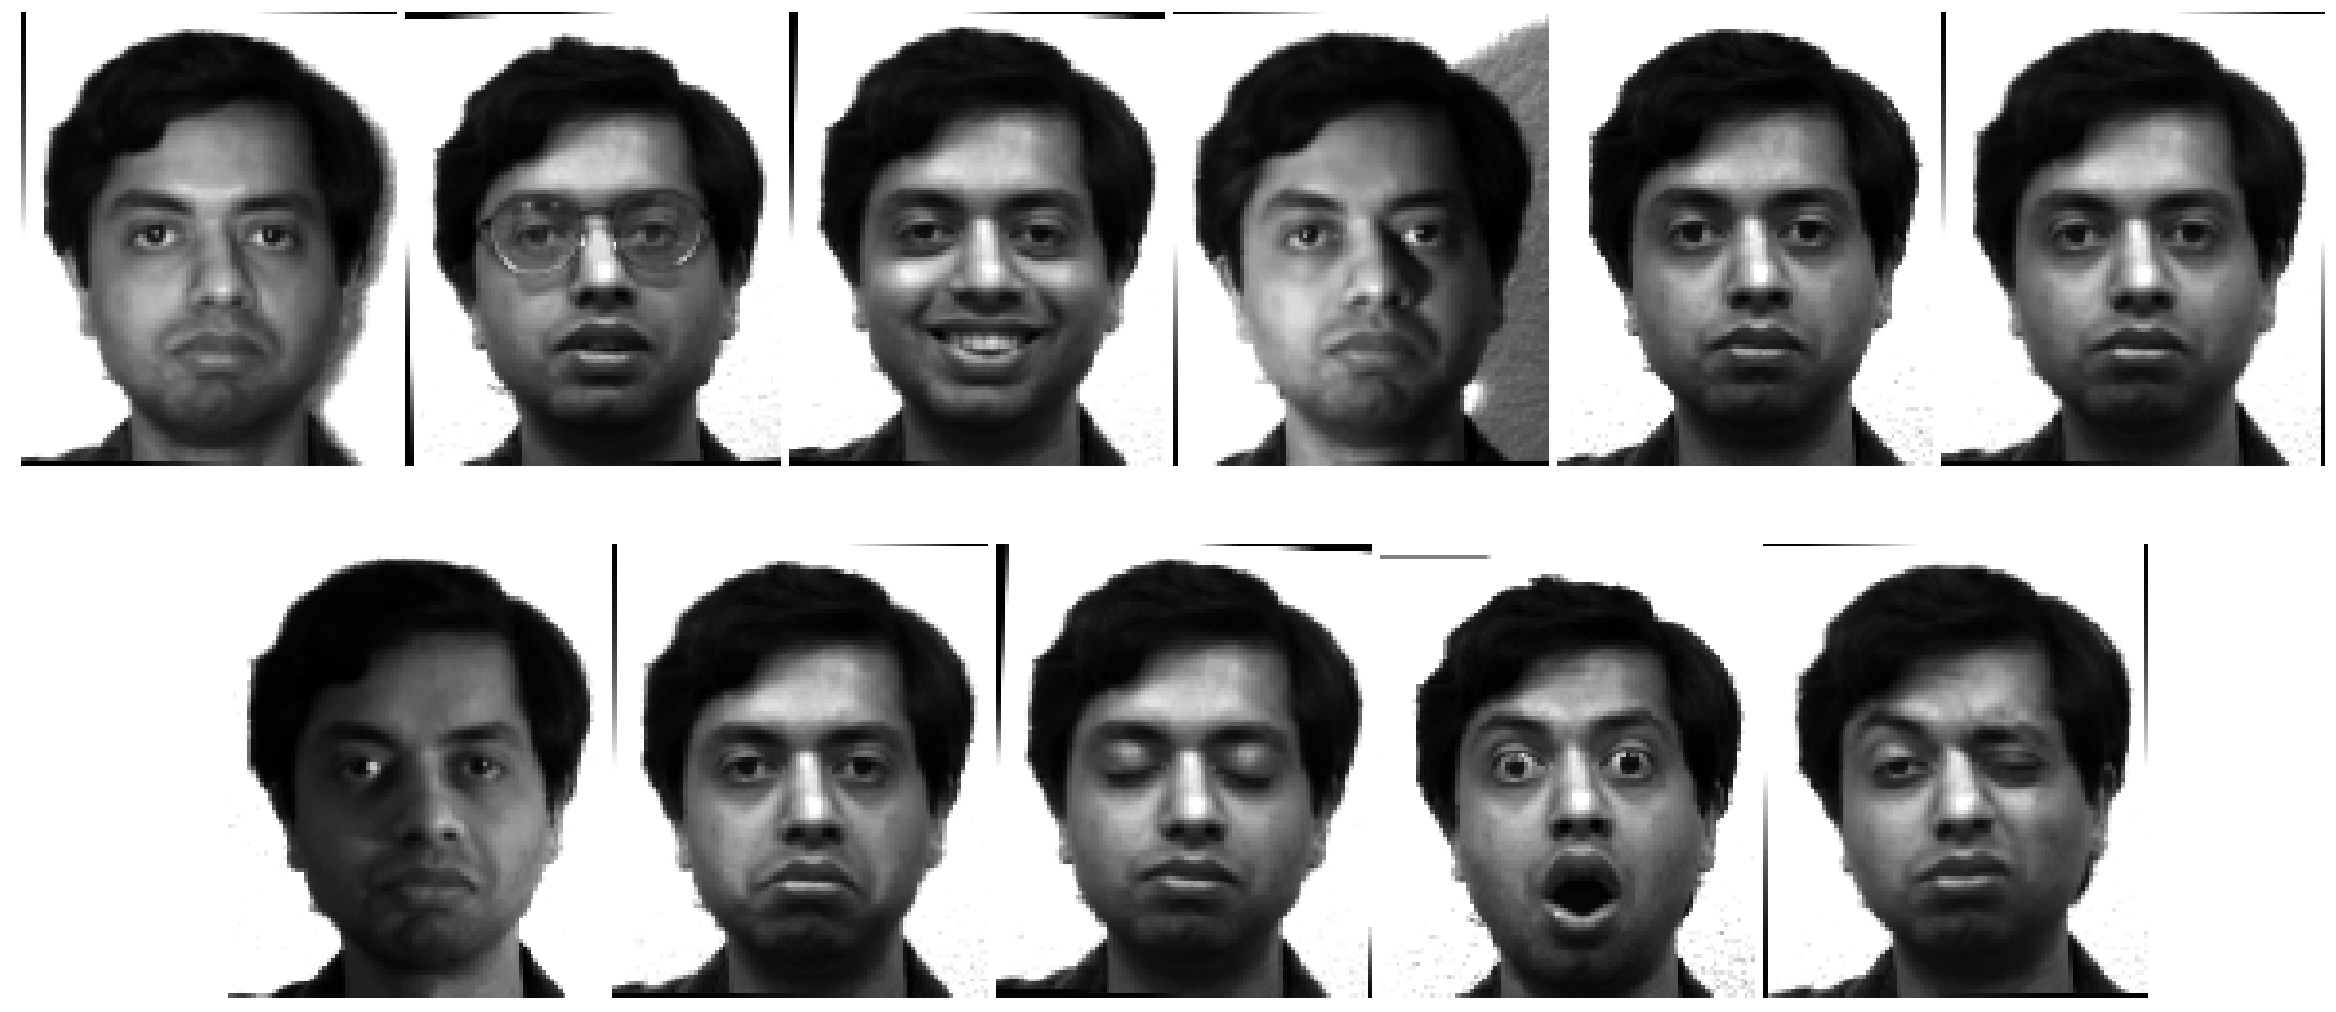
\includegraphics[width = \textwidth]{Chapters/content/28_pca2/latex/yaleb_exs.pdf}
    \caption[]{Ví dụ về ảnh của một người trong Yale Face Database.}
    \label{fig:28_1}
\end{figure}

Ta thấy rằng số chiều dữ liệu $116 \times 98 = 11368$ là một số khá
lớn. Tuy nhiên, vì chỉ có tổng cộng $15 \times 11 = 165$ bức ảnh nên ta có thể
nén các bức ảnh này về dữ liệu mới có chiều nhỏ hơn 165. Trong ví dụ này, chúng
ta chọn $K = 100$.

Dưới đây là đoạn code thực hiện PCA cho toàn bộ dữ liệu. Ở đây, PCA trong \pythoninline{sklearn} được sử dụng:
\newpage
\begin{lstlisting}[language=Python]
    from sklearn.decomposition import PCA
    import numpy as np
    import scipy.misc                  # for loading image
    from matplotlib.pyplot import imread
    np.random.seed(1)
    
    # filename structure
    path = 'YALE/unpadded/'  # path to the database
    ids = range(1, 16)  # 15 persons
    states = ['centerlight', 'glasses', 'happy', 'leftlight',
              'noglasses', 'normal', 'rightlight', 'sad',
              'sleepy', 'surprised', 'wink']
    prefix = 'subject'
    surfix = '.pgm'
    # data dimension
    h, w, K = 116, 98, 100  # hight, weight, new dim
    D = h * w
    N = len(states)*15
    # collect all data
    X = np.zeros((D, N))
    cnt = 0
    for person_id in range(1, 16):
        for state in states:
            fn = path + prefix + str(person_id).zfill(2) + '.' + state + surfix
            print(fn)
            X[:, cnt] = imread(fn).reshape(D)
            # misc.imread
            cnt += 1
    
    # Doing PCA, note that each row is a datapoint
    pca = PCA(n_components=K)  # K = 100
    pca.fit(X.T)
    # projection matrix
    U = pca.components_.T
    
\end{lstlisting}

Trong dòng \pythoninline{pca = PCA(n_components=K)}, nếu
\pythoninline{n_components} là một số thực trong khoảng $(0, 1)$, PCA sẽ thực
hiện việc tìm $K$ dựa trên biểu thức~\eqref{eqn:28_6}.

% ******************************************************************************
\begin{figure}[t]
    \centering
    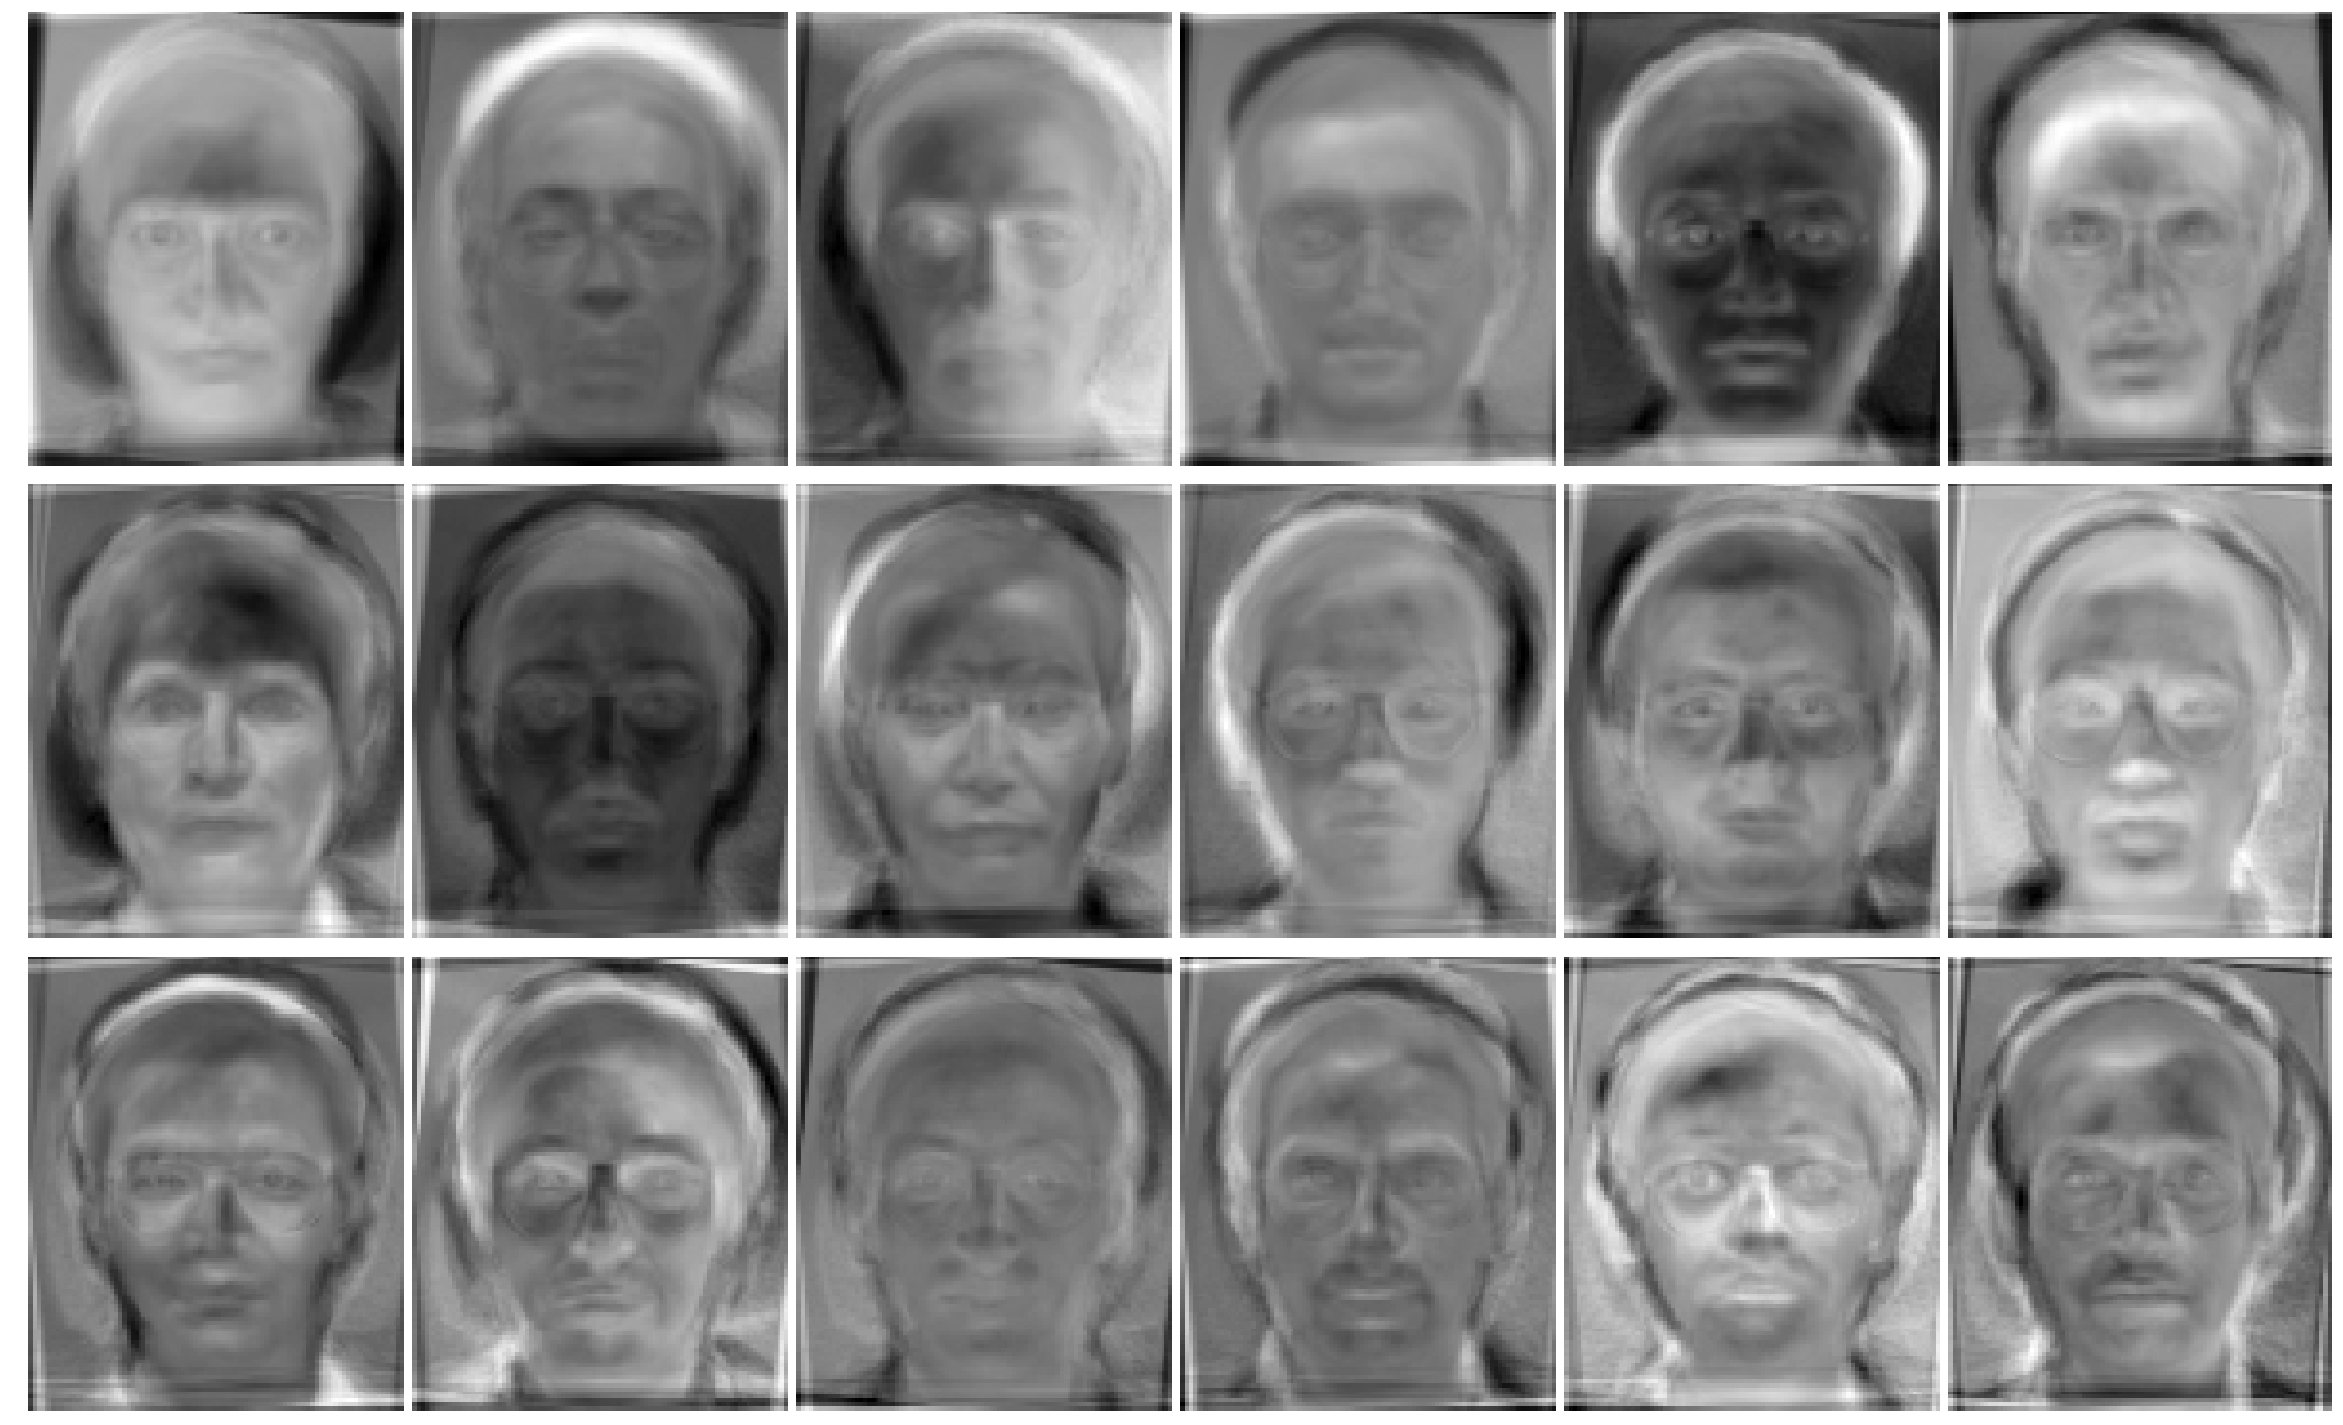
\includegraphics[width = \textwidth]{Chapters/content/28_pca2/latex/yaleb_eig.pdf}
    \caption[]{Các eigenfaces tìm được bằng PCA.}
    \label{fig:28_2}
\end{figure}
% ******************************************************************************

Hình \ref{fig:28_2} biểu diễn 18 vector riêng đầu tiên (18 cột đầu tiên của
$\bU_k$) tìm được bằng PCA. Các vector đã được \pythoninline{reshape} về cùng
kích thước như các bức ảnh gốc. Nhận thấy các
vector thu được ít nhiều mang thông tin của mặt người. Thực tế, một khuôn mặt
gốc sẽ được xấp xỉ như tổng có trọng số của các {khuôn mặt} này. Vì các
vector riêng này đóng vai trò như cơ sở của không gian mới với ít chiều hơn,
chúng còn được gọi là \textit{khuôn mặt riêng} hoặc \textit{khuôn mặt chính}. Từ \textit{chính} được dùng vì nó đi kèm với văn cảnh
của \textit{phân tích thành phần chính}.
% ******************************************************************************
\begin{figure}[t]
    \centering
    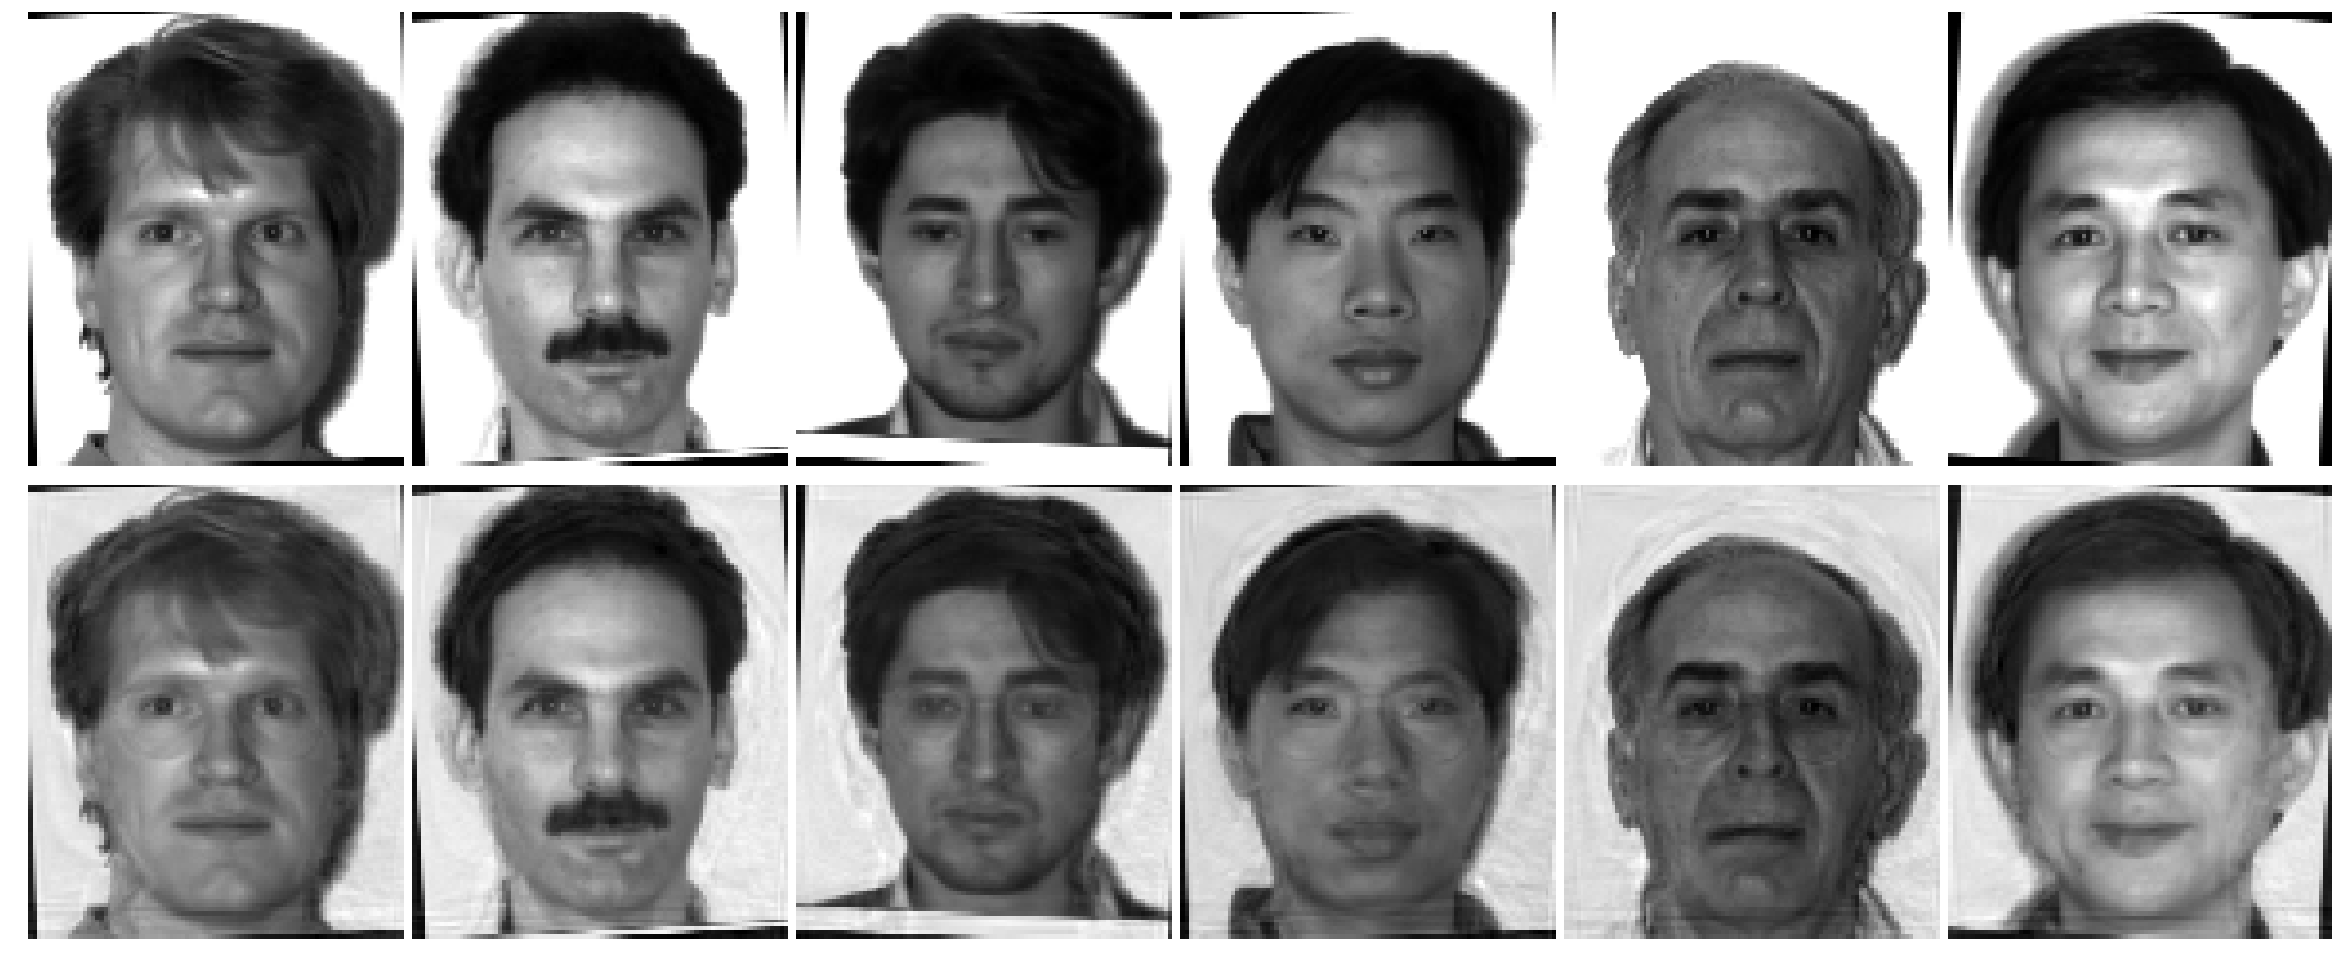
\includegraphics[width = \textwidth]{Chapters/content/28_pca2/latex/yaleb_ori_res.pdf}
    \caption[]{Hàng trên: các ảnh gốc. Hàng dưới: các ảnh được tái tạo dùng khuôn mặt riêng. Ảnh ở hàng dưới có nhiễu nhưng vẫn mang những đặc điểm riêng mà mắt người có thể phân biệt được.}
    \label{fig:28_3}
\end{figure}
% ******************************************************************************

Để xem mức độ hiệu quả của phương pháp này, chúng ta  minh hoạ các bức ảnh gốc và các bức ảnh được xấp xỉ bằng PCA như trên
Hình~\ref{fig:28_3}. Các khuôn mặt nhận được vẫn mang khá đầy đủ thông tin của
các khuôn mặt gốc. Đáng chú ý hơn, các khuôn mặt trong hàng dưới được suy ra
từ một vector 100 chiều, so với 11368 chiều như ở hàng trên.




% Phần còn lại của source code có thể được tìm thấy \href{https://github.com/tiepvupsu/tiepvupsu.github.io/blob/master/assets/28_pca2/python/EigenFaces.ipynb}{tại đây}.

\subsection{Dò tìm điểm bất thường}
Ngoài các ứng dụng về nén và phân loại, PCA còn được sử dụng trong nhiều lĩnh
vực khác. \textit{Dò tìm điểm bất thường} (abnormal detection hoặc {outlier
    detection}) là một trong số đó~\cite{shyu2003novel,lakhina2004diagnosing}.

Ý tưởng cơ bản là giả sử tồn tại một không gian con mà các sự kiện bình thường
nằm gần trong khi các sự kiện bất thường nằm xa không gian con đó. Hơn nữa, số
sự kiện bất thường có một tỉ lệ nhỏ. Như vậy, PCA có thể được sử dụng trên toàn
bộ dữ liệu để tìm ra các thành phần chính, từ đó suy ra không gian con mà các điểm bình thường nằm gần.
Việc xác định một điểm là bình thường hay bất thường được xác định bằng cách đo
khoảng cách từ điểm đó tới không gian con tìm được. Hình~\ref{fig:28_4} minh hoạ
cho việc xác định các sự kiện bất thường bằng PCA.

\begin{figure}[t]
    % caption on side

    \floatbox[{\capbeside\thisfloatsetup{capbesideposition={right,top},capbesidewidth=6.5cm}}]{figure}[\FBwidth]
    {\caption{ PCA cho bài toán dò tìm điểm bất thường. Giả sử
    các sự kiện {bình thường} chiếm đa số và nằm gần  một không
    gian con nào đó. Khi đó, nếu làm PCA trên toàn bộ dữ liệu, không gian con
    thu được gần với không gian con của tập các sự kiện {bình thường}.
    Lúc này, các
    điểm hình tròn to đậm hơn có thể được coi là các sự kiện {bất thường} vì chúng nằm xa không gian con chính.}
    \label{fig:28_4}}
    { % figure here
    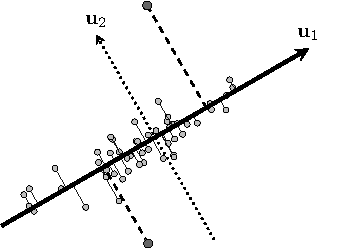
\includegraphics[width=.45\textwidth]{Chapters/content/28_pca2/latex/abnormal.pdf}
    }
\end{figure}


\section{Kết luận}
\begin{itemize}
    \item PCA là phương pháp giảm chiều dữ liệu dựa trên việc tối đa lượng
          thông tin được giữ lại. Lượng thông tin được giữ lại được đo bằng tổng các
          phương sai trên mỗi thành phần của dữ liệu. Lượng dữ liệu sẽ được giữ lại nhiều
          nhất khi các chiều dữ liệu còn lại tương ứng với các vector riêng của trị riêng
          lớn nhất của ma trận hiệp phương sai.

    \item Với các bài toán quy mô lớn, đôi khi việc tính toán trên toàn bộ dữ liệu
          là không khả thi vì vấn đề bộ nhớ. Giải pháp là thực hiện PCA lần đầu
          trên một tập con dữ liệu vừa với bộ nhớ, sau đó lấy một tập con khác để {từ từ} (\textit{incrementally}) cập nhật nghiệm của PCA tới khi hội
          tụ. Ý tưởng này khá giống với mini-batch gradient descent, và được gọi là
          incremental PCA~\cite{zhao2006novel}.


\end{itemize}



\backmatter%%%%%%%%%%%%%%%%%%%%%%%%%%%%%%%%%%%%%%%%%%%%%%%%%%%%%%%
\medskip
\bibliographystyle{abbrv}
\bibliography{refs}

% \printindex
\end{document}
